\refstepcounter{section}
\section*{Lecture 09: More on Ising Model}
\addcontentsline{toc}{section}{Lecture 09: More on Ising Model}
We have predicted a phase transition for the Ising model using mean-field approximation. However, the approximation seems to be inconsistent on many grounds, working well for higher dimensions and long-range interactions. It predicted that in 1D too, Ising model has a spontaneous magnetisation at some finite temperature which cannot be. Even though we have solved the Ising system for dimension $d=1$ in appendix. \ref{append:ising1d} (and it has been painfully solved by many stalwarts for $d=2$ case too), let us see some arguments on why phase transitions cannot occur for 1D but it is possible in 2D Ising system. 
\subsection{Phase Transition in 1D Ising System}
We will show that for $T>0$ in $d=1$ zero-field Ising Model, there exists no \textit{long-range order}. Consider the ground state of the Ising model at $T=0$, which is \textit{ordered}, with all spins aligned in the same direction. Under open boundary conditions, this configuration has minimum energy $E\tund{0} = -J(N-1)$.
\begin{figure}[H]
    \centering 
    \tikzset{every picture/.style={line width=0.75pt}} %set default line width to 0.75pt        

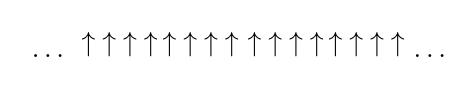
\begin{tikzpicture}[x=0.75pt,y=0.75pt,yscale=-1,xscale=1]
%uncomment if require: \path (0,241); %set diagram left start at 0, and has height of 241


% Text Node
\draw (96,134.4) node [anchor=north west][inner sep=0.75pt]    {$\ldots $};

\draw (120,123.4) node [anchor=north west][inner sep=0.75pt]    {$\uparrow $};
% Text Node
\draw (140,123.4) node [anchor=north west][inner sep=0.75pt]    {$\uparrow $};
% Text Node
\draw (130,123.4) node [anchor=north west][inner sep=0.75pt]    {$\uparrow $};
% Text Node
\draw (150,123.4) node [anchor=north west][inner sep=0.75pt]    {$\uparrow $};
% Text Node
\draw (159,123.4) node [anchor=north west][inner sep=0.75pt]    {$\uparrow $};
% Text Node
\draw (179,123.4) node [anchor=north west][inner sep=0.75pt]    {$\uparrow $};
% Text Node
\draw (169,123.4) node [anchor=north west][inner sep=0.75pt]    {$\uparrow $};
% Text Node
\draw (189,123.4) node [anchor=north west][inner sep=0.75pt]    {$\uparrow $};
% Text Node
\draw (200,123.4) node [anchor=north west][inner sep=0.75pt]    {$\uparrow $};
% Text Node
\draw (220,123.4) node [anchor=north west][inner sep=0.75pt]    {$\uparrow $};
% Text Node
\draw (210,123.4) node [anchor=north west][inner sep=0.75pt]    {$\uparrow $};
% Text Node
\draw (230,123.4) node [anchor=north west][inner sep=0.75pt]    {$\uparrow $};
% Text Node
\draw (239,123.4) node [anchor=north west][inner sep=0.75pt]    {$\uparrow $};
% Text Node
\draw (259,123.4) node [anchor=north west][inner sep=0.75pt]    {$\uparrow $};
% Text Node
\draw (249,123.4) node [anchor=north west][inner sep=0.75pt]    {$\uparrow $};
% Text Node
\draw (269,123.4) node [anchor=north west][inner sep=0.75pt]    {$\uparrow $};

\draw (280,134.4) node [anchor=north west][inner sep=0.75pt]    {$\ldots $};



\end{tikzpicture}
\end{figure}
\noindent
The above configuration has entropy $S=0$, since all the spins are aligned. Hence, the free energy of the system is $F\tund{grnd}=E-TS = -J(N-1)$.\\[0.2cm] On increasing the temperature, the spins flips randomly due to interactions and this increases the energy of the system (since the interaction term is $-J(-1) = +J$ only if neighbouring spins are oppositely aligned). We need to check whether this destroys the long-range order. Now, consider a configuration with one \textit{domain wall}\footnote{In simple terms, a domain wall is an imaginary boundary which separates \textit{domains}. Domains are regions with the same kind of spins, that is, all up or all down. } introduced at some point in the Ising chain, as shown in red below. 
\begin{figure}[H]
    \centering 
\tikzset{every picture/.style={line width=0.75pt}} %set default line width to 0.75pt        

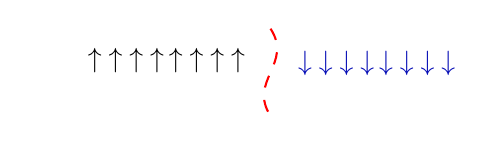
\begin{tikzpicture}[x=0.75pt,y=0.75pt,yscale=-1,xscale=1]
%uncomment if require: \path (0,241); %set diagram left start at 0, and has height of 241

%Shape: Boxed Bezier Curve [id:dp7848819814242627] 
\draw [color={rgb, 255:red, 255; green, 0; blue, 0 }  ,draw opacity=1 ] [dash pattern={on 4.5pt off 4.5pt}]  (197.51,67.6) .. controls (208.5,84.4) and (186.52,92.8) .. (197.51,109.6) ;

% Text Node
\draw (108,75.57) node [anchor=north west][inner sep=0.75pt]    {$\uparrow $};
% Text Node
\draw (128,75.57) node [anchor=north west][inner sep=0.75pt]    {$\uparrow $};
% Text Node
\draw (118,75.57) node [anchor=north west][inner sep=0.75pt]    {$\uparrow $};
% Text Node
\draw (138,75.57) node [anchor=north west][inner sep=0.75pt]    {$\uparrow $};
% Text Node
\draw (147,75.57) node [anchor=north west][inner sep=0.75pt]    {$\uparrow $};
% Text Node
\draw (167,75.57) node [anchor=north west][inner sep=0.75pt]    {$\uparrow $};
% Text Node
\draw (157,75.57) node [anchor=north west][inner sep=0.75pt]    {$\uparrow $};
% Text Node
\draw (177,75.57) node [anchor=north west][inner sep=0.75pt]    {$\uparrow $};
% Text Node
\draw (219,91.77) node [anchor=north east][inner sep=0.75pt]  [color={rgb, 255:red, 7; green, 14; blue, 182 }  ,opacity=1 ,rotate=-180,xscale=-1]  {$\uparrow $};
% Text Node
\draw (239,91.77) node [anchor=north east][inner sep=0.75pt]  [color={rgb, 255:red, 7; green, 14; blue, 182 }  ,opacity=1 ,rotate=-180,xscale=-1]  {$\uparrow $};
% Text Node
\draw (229,91.77) node [anchor=north east][inner sep=0.75pt]  [color={rgb, 255:red, 7; green, 14; blue, 182 }  ,opacity=1 ,rotate=-180,xscale=-1]  {$\uparrow $};
% Text Node
\draw (249,91.77) node [anchor=north east][inner sep=0.75pt]  [color={rgb, 255:red, 7; green, 14; blue, 182 }  ,opacity=1 ,rotate=-180,xscale=-1]  {$\uparrow $};
% Text Node
\draw (258,91.77) node [anchor=north east][inner sep=0.75pt]  [color={rgb, 255:red, 7; green, 14; blue, 182 }  ,opacity=1 ,rotate=-180,xscale=-1]  {$\uparrow $};
% Text Node
\draw (278,91.77) node [anchor=north east][inner sep=0.75pt]  [color={rgb, 255:red, 7; green, 14; blue, 182 }  ,opacity=1 ,rotate=-180,xscale=-1]  {$\uparrow $};
% Text Node
\draw (268,91.77) node [anchor=north east][inner sep=0.75pt]  [color={rgb, 255:red, 7; green, 14; blue, 182 }  ,opacity=1 ,rotate=-180,xscale=-1]  {$\uparrow $};
% Text Node
\draw (288,91.77) node [anchor=north east][inner sep=0.75pt]  [color={rgb, 255:red, 7; green, 14; blue, 182 }  ,opacity=1 ,rotate=-180,xscale=-1]  {$\uparrow $};
% Text Node
\draw (81,87.4) node [anchor=north west][inner sep=0.75pt]    {$\dotsc $};
% Text Node
\draw (288,84.4) node [anchor=north west][inner sep=0.75pt]  [color={rgb, 255:red, 19; green, 101; blue, 198 }  ,opacity=1 ]  {$\dotsc $};


\end{tikzpicture}
\end{figure}
\noindent
Introducing the domain wall increases the energy, due to the spins on either side of the domain wall.
$$E\tund{dw}= -J(N_+-1) -J(N_- -1) -J (-1) = -J(N-1)+2J$$
Thus introducing one domain wall incurs a cost of $\Delta E = 2J$. Now, since there are $N$ spins, this domain wall can be placed at any of the $(N-1)$ positions. Then the entropy of the system with one domain wall is $S=\kb \ln (N-1)$ and the free energy is $F\tund{dw} = -J(N-1) + 2J - \kb T\ln (N-1)$. The change in free energy is, 
$$\Delta  F= F\tund{dw} - F\tund{grnd} = 2J - \kb T\ln (N-1)$$
In the thermodynamic limit $N\to \infty$ which implies that $\Delta F \to -\infty$. The system can always lower the free energy by creating a domain wall for any temperature $T>0$. In fact, the free energy is further lowered by introducing arbitrary number of domain walls, untill no domains remain at all. This implies that the long-ranged order is unstable and there is no spontaneous magnetisation at any finite temperature in the zero-field $d=1$ Ising model. 
\subsection{Phase Transition in 2D Ising System ( Peirls' Argument)}
The situation becomes a bit different for $d=2$ Ising model. To prove the existence of phase transition at a finite temperature in $d=2$, consider a case where all the outer layer spins in the lattice are of the same type, say $\uparrow$. Now, consider the spin in the center of the lattice, highlighted yellow in Fig. \ref{peirl1}.
\begin{figure}[H]
    \centering 
    

\tikzset{every picture/.style={line width=0.75pt}} %set default line width to 0.75pt        

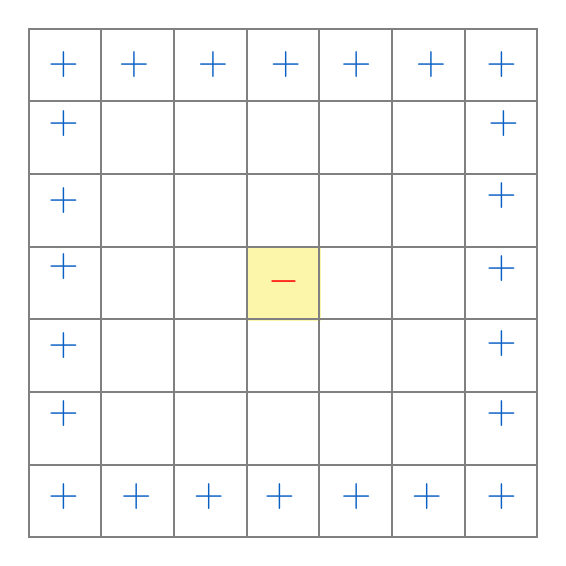
\begin{tikzpicture}[x=0.75pt,y=0.75pt,yscale=-1,xscale=1]
%uncomment if require: \path (0,300); %set diagram left start at 0, and has height of 300

%Shape: Square [id:dp7013067236152065] 
\draw  [draw opacity=0][fill={rgb, 255:red, 248; green, 231; blue, 28 }  ,fill opacity=0.37 ] (275,134.55) -- (310.68,134.55) -- (310.68,170.23) -- (275,170.23) -- cycle ;
%Shape: Grid [id:dp007204021057609311] 
\draw  [draw opacity=0] (170,29.55) -- (415,29.55) -- (415,274.55) -- (170,274.55) -- cycle ; \draw  [color={rgb, 255:red, 128; green, 128; blue, 128 }  ,draw opacity=1 ] (205,29.55) -- (205,274.55)(240,29.55) -- (240,274.55)(275,29.55) -- (275,274.55)(310,29.55) -- (310,274.55)(345,29.55) -- (345,274.55)(380,29.55) -- (380,274.55) ; \draw  [color={rgb, 255:red, 128; green, 128; blue, 128 }  ,draw opacity=1 ] (170,64.55) -- (415,64.55)(170,99.55) -- (415,99.55)(170,134.55) -- (415,134.55)(170,169.55) -- (415,169.55)(170,204.55) -- (415,204.55)(170,239.55) -- (415,239.55) ; \draw  [color={rgb, 255:red, 128; green, 128; blue, 128 }  ,draw opacity=1 ] (170,29.55) -- (415,29.55) -- (415,274.55) -- (170,274.55) -- cycle ;

% Text Node
\draw (178,39) node [anchor=north west][inner sep=0.75pt]  [font=\Large,color={rgb, 255:red, 9; green, 96; blue, 196 }  ,opacity=1 ]  {$+$};
% Text Node
\draw (212,39) node [anchor=north west][inner sep=0.75pt]  [font=\Large,color={rgb, 255:red, 9; green, 96; blue, 196 }  ,opacity=1 ]  {$+$};
% Text Node
\draw (250,39) node [anchor=north west][inner sep=0.75pt]  [font=\Large,color={rgb, 255:red, 9; green, 96; blue, 196 }  ,opacity=1 ]  {$+$};
% Text Node
\draw (285,39) node [anchor=north west][inner sep=0.75pt]  [font=\Large,color={rgb, 255:red, 9; green, 96; blue, 196 }  ,opacity=1 ]  {$+$};
% Text Node
\draw (319,39) node [anchor=north west][inner sep=0.75pt]  [font=\Large,color={rgb, 255:red, 9; green, 96; blue, 196 }  ,opacity=1 ]  {$+$};
% Text Node
\draw (355,39) node [anchor=north west][inner sep=0.75pt]  [font=\Large,color={rgb, 255:red, 9; green, 96; blue, 196 }  ,opacity=1 ]  {$+$};
% Text Node
\draw (389,39) node [anchor=north west][inner sep=0.75pt]  [font=\Large,color={rgb, 255:red, 9; green, 96; blue, 196 }  ,opacity=1 ]  {$+$};
% Text Node
\draw (390,67.4) node [anchor=north west][inner sep=0.75pt]  [font=\Large,color={rgb, 255:red, 9; green, 96; blue, 196 }  ,opacity=1 ]  {$+$};
% Text Node
\draw (389,102.4) node [anchor=north west][inner sep=0.75pt]  [font=\Large,color={rgb, 255:red, 9; green, 96; blue, 196 }  ,opacity=1 ]  {$+$};
% Text Node
\draw (389,137.4) node [anchor=north west][inner sep=0.75pt]  [font=\Large,color={rgb, 255:red, 9; green, 96; blue, 196 }  ,opacity=1 ]  {$+$};
% Text Node
\draw (389,173.4) node [anchor=north west][inner sep=0.75pt]  [font=\Large,color={rgb, 255:red, 9; green, 96; blue, 196 }  ,opacity=1 ]  {$+$};
% Text Node
\draw (389,207.4) node [anchor=north west][inner sep=0.75pt]  [font=\Large,color={rgb, 255:red, 9; green, 96; blue, 196 }  ,opacity=1 ]  {$+$};
% Text Node
\draw (389,247.4) node [anchor=north west][inner sep=0.75pt]  [font=\Large,color={rgb, 255:red, 9; green, 96; blue, 196 }  ,opacity=1 ]  {$+$};
% Text Node
\draw (353,247.4) node [anchor=north west][inner sep=0.75pt]  [font=\Large,color={rgb, 255:red, 9; green, 96; blue, 196 }  ,opacity=1 ]  {$+$};
% Text Node
\draw (319,247.4) node [anchor=north west][inner sep=0.75pt]  [font=\Large,color={rgb, 255:red, 9; green, 96; blue, 196 }  ,opacity=1 ]  {$+$};
% Text Node
\draw (282,247.4) node [anchor=north west][inner sep=0.75pt]  [font=\Large,color={rgb, 255:red, 9; green, 96; blue, 196 }  ,opacity=1 ]  {$+$};
% Text Node
\draw (248,247.4) node [anchor=north west][inner sep=0.75pt]  [font=\Large,color={rgb, 255:red, 9; green, 96; blue, 196 }  ,opacity=1 ]  {$+$};
% Text Node
\draw (213,247.4) node [anchor=north west][inner sep=0.75pt]  [font=\Large,color={rgb, 255:red, 9; green, 96; blue, 196 }  ,opacity=1 ]  {$+$};
% Text Node
\draw (178,247.4) node [anchor=north west][inner sep=0.75pt]  [font=\Large,color={rgb, 255:red, 9; green, 96; blue, 196 }  ,opacity=1 ]  {$+$};
% Text Node
\draw (178,207.4) node [anchor=north west][inner sep=0.75pt]  [font=\Large,color={rgb, 255:red, 9; green, 96; blue, 196 }  ,opacity=1 ]  {$+$};
% Text Node
\draw (178,67.4) node [anchor=north west][inner sep=0.75pt]  [font=\Large,color={rgb, 255:red, 9; green, 96; blue, 196 }  ,opacity=1 ]  {$+$};
% Text Node
\draw (178,104.4) node [anchor=north west][inner sep=0.75pt]  [font=\Large,color={rgb, 255:red, 9; green, 96; blue, 196 }  ,opacity=1 ]  {$+$};
% Text Node
\draw (178,136.4) node [anchor=north west][inner sep=0.75pt]  [font=\Large,color={rgb, 255:red, 9; green, 96; blue, 196 }  ,opacity=1 ]  {$+$};
% Text Node
\draw (178,174.4) node [anchor=north west][inner sep=0.75pt]  [font=\Large,color={rgb, 255:red, 9; green, 96; blue, 196 }  ,opacity=1 ]  {$+$};
% Text Node
\draw (284,143.4) node [anchor=north west][inner sep=0.75pt]  [font=\Large,color={rgb, 255:red, 255; green, 0; blue, 0 }  ,opacity=1 ]  {$-$};


\end{tikzpicture}

    \caption{2D Ising lattice; the outer layer have all same spins while the center spin is oppositely aligned with the outer spins.}
    \label{peirl1}
\end{figure}
\noindent
If there is spontaneous magnetisation at some finite temperature, then the probability of the center spin to be oppositely aligned to the outer spins become zero (since the lattice becomes \textit{ordered}). Also, note that the central spin is not particularly important and is just a representative of the bulk spin. 
\begin{figure}[H]
    \centering 
    

\tikzset{every picture/.style={line width=0.75pt}} %set default line width to 0.75pt        

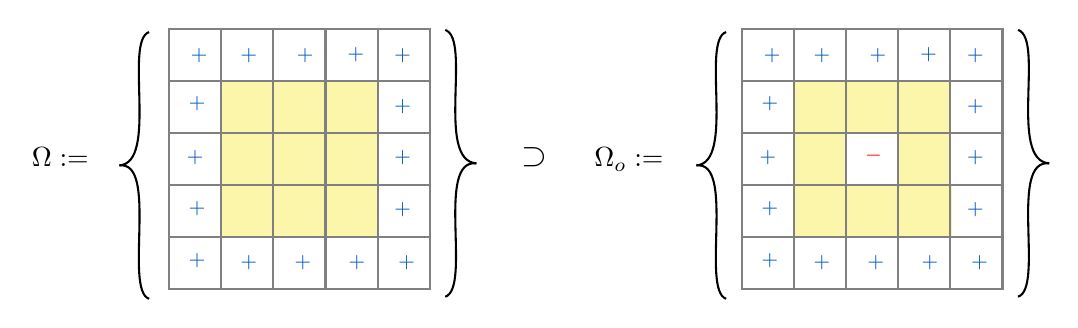
\begin{tikzpicture}[x=0.75pt,y=0.75pt,yscale=-1,xscale=1]
%uncomment if require: \path (0,300); %set diagram left start at 0, and has height of 300

%Shape: Rectangle [id:dp23729130462669978] 
\draw  [draw opacity=0][fill={rgb, 255:red, 248; green, 231; blue, 28 }  ,fill opacity=0.37 ] (456.98,76.59) -- (482.07,76.59) -- (482.07,101.69) -- (456.98,101.69) -- cycle ;
%Shape: Rectangle [id:dp5061265863591148] 
\draw  [draw opacity=0][fill={rgb, 255:red, 248; green, 231; blue, 28 }  ,fill opacity=0.37 ] (406.78,76.59) -- (431.88,76.59) -- (431.88,101.69) -- (406.78,101.69) -- cycle ;
%Shape: Rectangle [id:dp8322890296325763] 
\draw  [draw opacity=0][fill={rgb, 255:red, 248; green, 231; blue, 28 }  ,fill opacity=0.37 ] (406.78,101.69) -- (482.68,101.69) -- (482.68,126.79) -- (406.78,126.79) -- cycle ;
%Shape: Rectangle [id:dp03842665382729815] 
\draw  [draw opacity=0][fill={rgb, 255:red, 248; green, 231; blue, 28 }  ,fill opacity=0.37 ] (406.78,51.5) -- (482.07,51.5) -- (482.07,76.59) -- (406.78,76.59) -- cycle ;
%Shape: Grid [id:dp6545635847552198] 
\draw  [draw opacity=0] (381.68,26.4) -- (507.17,26.4) -- (507.17,151.89) -- (381.68,151.89) -- cycle ; \draw  [color={rgb, 255:red, 128; green, 128; blue, 128 }  ,draw opacity=1 ] (406.78,26.4) -- (406.78,151.89)(431.88,26.4) -- (431.88,151.89)(456.98,26.4) -- (456.98,151.89)(482.07,26.4) -- (482.07,151.89) ; \draw  [color={rgb, 255:red, 128; green, 128; blue, 128 }  ,draw opacity=1 ] (381.68,51.5) -- (507.17,51.5)(381.68,76.59) -- (507.17,76.59)(381.68,101.69) -- (507.17,101.69)(381.68,126.79) -- (507.17,126.79) ; \draw  [color={rgb, 255:red, 128; green, 128; blue, 128 }  ,draw opacity=1 ] (381.68,26.4) -- (507.17,26.4) -- (507.17,151.89) -- (381.68,151.89) -- cycle ;
%Shape: Rectangle [id:dp9604221987758147] 
\draw  [draw opacity=0][fill={rgb, 255:red, 248; green, 231; blue, 28 }  ,fill opacity=0.37 ] (130.78,51.5) -- (206.07,51.5) -- (206.07,126.79) -- (130.78,126.79) -- cycle ;
%Shape: Grid [id:dp23793276171823607] 
\draw  [draw opacity=0] (105.68,26.4) -- (231.17,26.4) -- (231.17,151.89) -- (105.68,151.89) -- cycle ; \draw  [color={rgb, 255:red, 128; green, 128; blue, 128 }  ,draw opacity=1 ] (130.78,26.4) -- (130.78,151.89)(155.88,26.4) -- (155.88,151.89)(180.98,26.4) -- (180.98,151.89)(206.07,26.4) -- (206.07,151.89) ; \draw  [color={rgb, 255:red, 128; green, 128; blue, 128 }  ,draw opacity=1 ] (105.68,51.5) -- (231.17,51.5)(105.68,76.59) -- (231.17,76.59)(105.68,101.69) -- (231.17,101.69)(105.68,126.79) -- (231.17,126.79) ; \draw  [color={rgb, 255:red, 128; green, 128; blue, 128 }  ,draw opacity=1 ] (105.68,26.4) -- (231.17,26.4) -- (231.17,151.89) -- (105.68,151.89) -- cycle ;
%Curve Lines [id:da19406680747920868] 
\draw    (96,28) .. controls (83.78,32.18) and (100.55,90.95) .. (81.68,92.27) ;
%Curve Lines [id:da5286592940064089] 
\draw    (96,156.53) .. controls (83.78,152.35) and (100.55,89.95) .. (81.68,92.27) ;

%Curve Lines [id:da8102843282113134] 
\draw    (238.68,27) .. controls (251.49,31.18) and (233.92,89.95) .. (253.68,91.27) ;
%Curve Lines [id:da7527697969478102] 
\draw    (238.68,155.53) .. controls (251.49,151.35) and (233.92,88.95) .. (253.68,91.27) ;

%Curve Lines [id:da98716542851002] 
\draw    (374,28) .. controls (361.78,32.18) and (378.55,90.95) .. (359.68,92.27) ;
%Curve Lines [id:da7361200068274598] 
\draw    (374,156.53) .. controls (361.78,152.35) and (378.55,89.95) .. (359.68,92.27) ;

%Curve Lines [id:da04921238856224297] 
\draw    (514.68,27) .. controls (527.49,31.18) and (509.92,89.95) .. (529.68,91.27) ;
%Curve Lines [id:da2525982723838034] 
\draw    (514.68,155.53) .. controls (527.49,151.35) and (509.92,88.95) .. (529.68,91.27) ;


% Text Node
\draw (488.54,34.36) node [anchor=north west][inner sep=0.75pt]  [font=\scriptsize,color={rgb, 255:red, 9; green, 96; blue, 196 }  ,opacity=1 ]  {$+$};
% Text Node
\draw (488.54,59.09) node [anchor=north west][inner sep=0.75pt]  [font=\scriptsize,color={rgb, 255:red, 9; green, 96; blue, 196 }  ,opacity=1 ]  {$+$};
% Text Node
\draw (488.54,83.38) node [anchor=north west][inner sep=0.75pt]  [font=\scriptsize,color={rgb, 255:red, 9; green, 96; blue, 196 }  ,opacity=1 ]  {$+$};
% Text Node
\draw (488.54,108.55) node [anchor=north west][inner sep=0.75pt]  [font=\scriptsize,color={rgb, 255:red, 9; green, 96; blue, 196 }  ,opacity=1 ]  {$+$};
% Text Node
\draw (490.54,134.28) node [anchor=north west][inner sep=0.75pt]  [font=\scriptsize,color={rgb, 255:red, 9; green, 96; blue, 196 }  ,opacity=1 ]  {$+$};
% Text Node
\draw (439.33,82.65) node [anchor=north west][inner sep=0.75pt]  [font=\scriptsize,color={rgb, 255:red, 255; green, 0; blue, 0 }  ,opacity=1 ]  {$-$};
% Text Node
\draw (465.98,33.8) node [anchor=north west][inner sep=0.75pt]  [font=\scriptsize,color={rgb, 255:red, 9; green, 96; blue, 196 }  ,opacity=1 ]  {$+$};
% Text Node
\draw (441.54,34.36) node [anchor=north west][inner sep=0.75pt]  [font=\scriptsize,color={rgb, 255:red, 9; green, 96; blue, 196 }  ,opacity=1 ]  {$+$};
% Text Node
\draw (414.54,34.36) node [anchor=north west][inner sep=0.75pt]  [font=\scriptsize,color={rgb, 255:red, 9; green, 96; blue, 196 }  ,opacity=1 ]  {$+$};
% Text Node
\draw (390.54,34.36) node [anchor=north west][inner sep=0.75pt]  [font=\scriptsize,color={rgb, 255:red, 9; green, 96; blue, 196 }  ,opacity=1 ]  {$+$};
% Text Node
\draw (389.54,57.36) node [anchor=north west][inner sep=0.75pt]  [font=\scriptsize,color={rgb, 255:red, 9; green, 96; blue, 196 }  ,opacity=1 ]  {$+$};
% Text Node
\draw (388.54,83.36) node [anchor=north west][inner sep=0.75pt]  [font=\scriptsize,color={rgb, 255:red, 9; green, 96; blue, 196 }  ,opacity=1 ]  {$+$};
% Text Node
\draw (389.54,108.36) node [anchor=north west][inner sep=0.75pt]  [font=\scriptsize,color={rgb, 255:red, 9; green, 96; blue, 196 }  ,opacity=1 ]  {$+$};
% Text Node
\draw (389.54,133.36) node [anchor=north west][inner sep=0.75pt]  [font=\scriptsize,color={rgb, 255:red, 9; green, 96; blue, 196 }  ,opacity=1 ]  {$+$};
% Text Node
\draw (414.54,134.36) node [anchor=north west][inner sep=0.75pt]  [font=\scriptsize,color={rgb, 255:red, 9; green, 96; blue, 196 }  ,opacity=1 ]  {$+$};
% Text Node
\draw (440.54,134.36) node [anchor=north west][inner sep=0.75pt]  [font=\scriptsize,color={rgb, 255:red, 9; green, 96; blue, 196 }  ,opacity=1 ]  {$+$};
% Text Node
\draw (466.54,134.36) node [anchor=north west][inner sep=0.75pt]  [font=\scriptsize,color={rgb, 255:red, 9; green, 96; blue, 196 }  ,opacity=1 ]  {$+$};
% Text Node
\draw (212.54,34.36) node [anchor=north west][inner sep=0.75pt]  [font=\scriptsize,color={rgb, 255:red, 9; green, 96; blue, 196 }  ,opacity=1 ]  {$+$};
% Text Node
\draw (212.54,59.09) node [anchor=north west][inner sep=0.75pt]  [font=\scriptsize,color={rgb, 255:red, 9; green, 96; blue, 196 }  ,opacity=1 ]  {$+$};
% Text Node
\draw (212.54,83.38) node [anchor=north west][inner sep=0.75pt]  [font=\scriptsize,color={rgb, 255:red, 9; green, 96; blue, 196 }  ,opacity=1 ]  {$+$};
% Text Node
\draw (212.54,108.55) node [anchor=north west][inner sep=0.75pt]  [font=\scriptsize,color={rgb, 255:red, 9; green, 96; blue, 196 }  ,opacity=1 ]  {$+$};
% Text Node
\draw (214.54,134.28) node [anchor=north west][inner sep=0.75pt]  [font=\scriptsize,color={rgb, 255:red, 9; green, 96; blue, 196 }  ,opacity=1 ]  {$+$};
% Text Node
\draw (189.98,33.8) node [anchor=north west][inner sep=0.75pt]  [font=\scriptsize,color={rgb, 255:red, 9; green, 96; blue, 196 }  ,opacity=1 ]  {$+$};
% Text Node
\draw (165.54,34.36) node [anchor=north west][inner sep=0.75pt]  [font=\scriptsize,color={rgb, 255:red, 9; green, 96; blue, 196 }  ,opacity=1 ]  {$+$};
% Text Node
\draw (138.54,34.36) node [anchor=north west][inner sep=0.75pt]  [font=\scriptsize,color={rgb, 255:red, 9; green, 96; blue, 196 }  ,opacity=1 ]  {$+$};
% Text Node
\draw (114.54,34.36) node [anchor=north west][inner sep=0.75pt]  [font=\scriptsize,color={rgb, 255:red, 9; green, 96; blue, 196 }  ,opacity=1 ]  {$+$};
% Text Node
\draw (113.54,57.36) node [anchor=north west][inner sep=0.75pt]  [font=\scriptsize,color={rgb, 255:red, 9; green, 96; blue, 196 }  ,opacity=1 ]  {$+$};
% Text Node
\draw (112.54,83.36) node [anchor=north west][inner sep=0.75pt]  [font=\scriptsize,color={rgb, 255:red, 9; green, 96; blue, 196 }  ,opacity=1 ]  {$+$};
% Text Node
\draw (113.54,108.36) node [anchor=north west][inner sep=0.75pt]  [font=\scriptsize,color={rgb, 255:red, 9; green, 96; blue, 196 }  ,opacity=1 ]  {$+$};
% Text Node
\draw (113.54,133.36) node [anchor=north west][inner sep=0.75pt]  [font=\scriptsize,color={rgb, 255:red, 9; green, 96; blue, 196 }  ,opacity=1 ]  {$+$};
% Text Node
\draw (138.54,134.36) node [anchor=north west][inner sep=0.75pt]  [font=\scriptsize,color={rgb, 255:red, 9; green, 96; blue, 196 }  ,opacity=1 ]  {$+$};
% Text Node
\draw (164.54,134.36) node [anchor=north west][inner sep=0.75pt]  [font=\scriptsize,color={rgb, 255:red, 9; green, 96; blue, 196 }  ,opacity=1 ]  {$+$};
% Text Node
\draw (190.54,134.36) node [anchor=north west][inner sep=0.75pt]  [font=\scriptsize,color={rgb, 255:red, 9; green, 96; blue, 196 }  ,opacity=1 ]  {$+$};
% Text Node
\draw (38,82.4) node [anchor=north west][inner sep=0.75pt]    {$\Omega :=$};
% Text Node
\draw (309,82.4) node [anchor=north west][inner sep=0.75pt]    {$\Omega _{o} :=$};
% Text Node
\draw (274,82.4) node [anchor=north west][inner sep=0.75pt]  [font=\large]  {$\supset $};


\end{tikzpicture}

\end{figure} 
\noindent
Now, consider $\Omega$ to be the set of all configurations where all the outer layers have spin $+$. Naturally, if we define $\Omega\tund{0}$ to be the set of all configurations where the central spin is $-$ and all the outer layers have spin $+$, we have $\Omega\tund{0}\subset \Omega$, as shown in the above figure. To have a phase transition is to show that the probability of any configuration $\{\sigma\} \in \Omega\tund{0} \to 0$ as $N\to \infty$. \\[0.2cm]
To show that, we define a \textit{shoreline} which is an imaginary closed loop separating $+$ spins from $-$ spins. So, along the boundary of the shoreline, we have all opposite spins on either side. A given shoreline thus separates spins $\sigma_i$ and $\sigma_j$ such that $\sigma_i\cdot \sigma_j = -1$. Note that, in the interior of the shoreline, there can be $+$ or $-$ spins.\\[0.2cm]
We define another set of configurations, $\Omega\tund{s}$ in which every configuration has the central spin to be $-$ and all the outer layers have spin $+$. In addition to it, there is a \textit{fixed} shoreline $S$ surrounding the central spin. Clearly, $\Omega\tund{s}\subset \Omega\tund{0}$
\begin{figure}[H]
    \centering 
    

\tikzset{every picture/.style={line width=0.75pt}} %set default line width to 0.75pt        

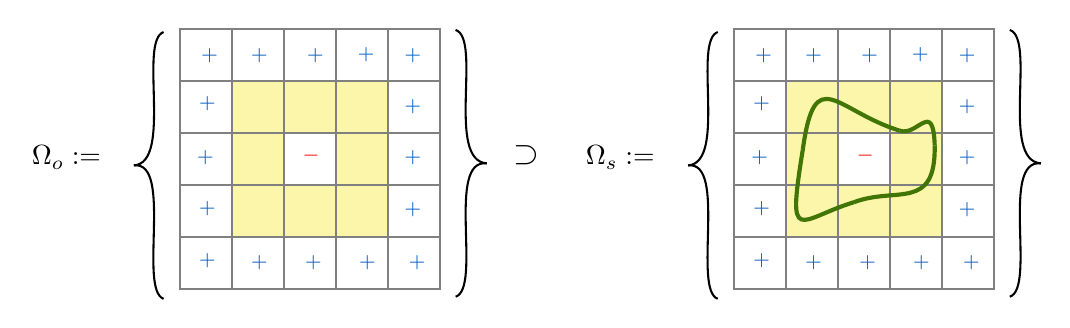
\begin{tikzpicture}[x=0.75pt,y=0.75pt,yscale=-1,xscale=1]
%uncomment if require: \path (0,192); %set diagram left start at 0, and has height of 192

%Shape: Rectangle [id:dp1875272590329995] 
\draw  [draw opacity=0][fill={rgb, 255:red, 248; green, 231; blue, 28 }  ,fill opacity=0.37 ] (288.98,76.59) -- (314.07,76.59) -- (314.07,101.69) -- (288.98,101.69) -- cycle ;
%Shape: Rectangle [id:dp45926838944511017] 
\draw  [draw opacity=0][fill={rgb, 255:red, 248; green, 231; blue, 28 }  ,fill opacity=0.37 ] (238.78,76.59) -- (263.88,76.59) -- (263.88,101.69) -- (238.78,101.69) -- cycle ;
%Shape: Rectangle [id:dp951208679037494] 
\draw  [draw opacity=0][fill={rgb, 255:red, 248; green, 231; blue, 28 }  ,fill opacity=0.37 ] (238.78,101.69) -- (314.68,101.69) -- (314.68,126.79) -- (238.78,126.79) -- cycle ;
%Shape: Rectangle [id:dp007344814580564685] 
\draw  [draw opacity=0][fill={rgb, 255:red, 248; green, 231; blue, 28 }  ,fill opacity=0.37 ] (238.78,51.5) -- (314.07,51.5) -- (314.07,76.59) -- (238.78,76.59) -- cycle ;
%Shape: Grid [id:dp3223419934026063] 
\draw  [draw opacity=0] (213.68,26.4) -- (339.17,26.4) -- (339.17,151.89) -- (213.68,151.89) -- cycle ; \draw  [color={rgb, 255:red, 128; green, 128; blue, 128 }  ,draw opacity=1 ] (238.78,26.4) -- (238.78,151.89)(263.88,26.4) -- (263.88,151.89)(288.98,26.4) -- (288.98,151.89)(314.07,26.4) -- (314.07,151.89) ; \draw  [color={rgb, 255:red, 128; green, 128; blue, 128 }  ,draw opacity=1 ] (213.68,51.5) -- (339.17,51.5)(213.68,76.59) -- (339.17,76.59)(213.68,101.69) -- (339.17,101.69)(213.68,126.79) -- (339.17,126.79) ; \draw  [color={rgb, 255:red, 128; green, 128; blue, 128 }  ,draw opacity=1 ] (213.68,26.4) -- (339.17,26.4) -- (339.17,151.89) -- (213.68,151.89) -- cycle ;
%Curve Lines [id:da008301583048880179] 
\draw    (206,28) .. controls (193.78,32.18) and (210.55,90.95) .. (191.68,92.27) ;
%Curve Lines [id:da5597728155003041] 
\draw    (206,156.53) .. controls (193.78,152.35) and (210.55,89.95) .. (191.68,92.27) ;

%Curve Lines [id:da02896941551177379] 
\draw    (346.68,27) .. controls (359.49,31.18) and (341.92,89.95) .. (361.68,91.27) ;
%Curve Lines [id:da9303782701504543] 
\draw    (346.68,155.53) .. controls (359.49,151.35) and (341.92,88.95) .. (361.68,91.27) ;

%Shape: Rectangle [id:dp8595008353400008] 
\draw  [draw opacity=0][fill={rgb, 255:red, 248; green, 231; blue, 28 }  ,fill opacity=0.37 ] (555.98,76.59) -- (581.07,76.59) -- (581.07,101.69) -- (555.98,101.69) -- cycle ;
%Shape: Rectangle [id:dp10897143783297769] 
\draw  [draw opacity=0][fill={rgb, 255:red, 248; green, 231; blue, 28 }  ,fill opacity=0.37 ] (505.78,76.59) -- (530.88,76.59) -- (530.88,101.69) -- (505.78,101.69) -- cycle ;
%Shape: Rectangle [id:dp8256281985192404] 
\draw  [draw opacity=0][fill={rgb, 255:red, 248; green, 231; blue, 28 }  ,fill opacity=0.37 ] (505.78,101.69) -- (581.68,101.69) -- (581.68,126.79) -- (505.78,126.79) -- cycle ;
%Shape: Rectangle [id:dp9508677694883004] 
\draw  [draw opacity=0][fill={rgb, 255:red, 248; green, 231; blue, 28 }  ,fill opacity=0.37 ] (505.78,51.5) -- (581.07,51.5) -- (581.07,76.59) -- (505.78,76.59) -- cycle ;
%Shape: Grid [id:dp6918715763510325] 
\draw  [draw opacity=0] (480.68,26.4) -- (606.17,26.4) -- (606.17,151.89) -- (480.68,151.89) -- cycle ; \draw  [color={rgb, 255:red, 128; green, 128; blue, 128 }  ,draw opacity=1 ] (505.78,26.4) -- (505.78,151.89)(530.88,26.4) -- (530.88,151.89)(555.98,26.4) -- (555.98,151.89)(581.07,26.4) -- (581.07,151.89) ; \draw  [color={rgb, 255:red, 128; green, 128; blue, 128 }  ,draw opacity=1 ] (480.68,51.5) -- (606.17,51.5)(480.68,76.59) -- (606.17,76.59)(480.68,101.69) -- (606.17,101.69)(480.68,126.79) -- (606.17,126.79) ; \draw  [color={rgb, 255:red, 128; green, 128; blue, 128 }  ,draw opacity=1 ] (480.68,26.4) -- (606.17,26.4) -- (606.17,151.89) -- (480.68,151.89) -- cycle ;
%Curve Lines [id:da6295844255433479] 
\draw    (473,28) .. controls (460.78,32.18) and (477.55,90.95) .. (458.68,92.27) ;
%Curve Lines [id:da968864494956809] 
\draw    (473,156.53) .. controls (460.78,152.35) and (477.55,89.95) .. (458.68,92.27) ;

%Curve Lines [id:da8514128320377528] 
\draw    (613.68,27) .. controls (626.49,31.18) and (608.92,89.95) .. (628.68,91.27) ;
%Curve Lines [id:da03483001801406849] 
\draw    (613.68,155.53) .. controls (626.49,151.35) and (608.92,88.95) .. (628.68,91.27) ;

%Curve Lines [id:da6944076159894066] 
\draw [color={rgb, 255:red, 65; green, 117; blue, 5 }  ,draw opacity=1 ][line width=1.5]    (513.94,84.76) .. controls (519.79,42.26) and (529.63,65.86) .. (560.53,75.49) ;
%Curve Lines [id:da04901172257911568] 
\draw [color={rgb, 255:red, 65; green, 117; blue, 5 }  ,draw opacity=1 ][line width=1.5]    (513.94,84.76) .. controls (506.21,132.25) and (511.69,118.26) .. (538.64,109.97) ;
%Curve Lines [id:da12532524491720676] 
\draw [color={rgb, 255:red, 65; green, 117; blue, 5 }  ,draw opacity=1 ][line width=1.5]    (538.64,109.97) .. controls (559.21,102.26) and (578.04,114.54) .. (577.5,82.61) ;
%Curve Lines [id:da17629004511076274] 
\draw [color={rgb, 255:red, 65; green, 117; blue, 5 }  ,draw opacity=1 ][line width=1.5]    (560.53,75.49) .. controls (569.08,78.76) and (576.78,59.92) .. (577.5,82.61) ;


% Text Node
\draw (320.54,34.36) node [anchor=north west][inner sep=0.75pt]  [font=\scriptsize,color={rgb, 255:red, 9; green, 96; blue, 196 }  ,opacity=1 ]  {$+$};
% Text Node
\draw (320.54,59.09) node [anchor=north west][inner sep=0.75pt]  [font=\scriptsize,color={rgb, 255:red, 9; green, 96; blue, 196 }  ,opacity=1 ]  {$+$};
% Text Node
\draw (320.54,83.38) node [anchor=north west][inner sep=0.75pt]  [font=\scriptsize,color={rgb, 255:red, 9; green, 96; blue, 196 }  ,opacity=1 ]  {$+$};
% Text Node
\draw (320.54,108.55) node [anchor=north west][inner sep=0.75pt]  [font=\scriptsize,color={rgb, 255:red, 9; green, 96; blue, 196 }  ,opacity=1 ]  {$+$};
% Text Node
\draw (322.54,134.28) node [anchor=north west][inner sep=0.75pt]  [font=\scriptsize,color={rgb, 255:red, 9; green, 96; blue, 196 }  ,opacity=1 ]  {$+$};
% Text Node
\draw (271.33,82.65) node [anchor=north west][inner sep=0.75pt]  [font=\scriptsize,color={rgb, 255:red, 255; green, 0; blue, 0 }  ,opacity=1 ]  {$-$};
% Text Node
\draw (297.98,33.8) node [anchor=north west][inner sep=0.75pt]  [font=\scriptsize,color={rgb, 255:red, 9; green, 96; blue, 196 }  ,opacity=1 ]  {$+$};
% Text Node
\draw (273.54,34.36) node [anchor=north west][inner sep=0.75pt]  [font=\scriptsize,color={rgb, 255:red, 9; green, 96; blue, 196 }  ,opacity=1 ]  {$+$};
% Text Node
\draw (246.54,34.36) node [anchor=north west][inner sep=0.75pt]  [font=\scriptsize,color={rgb, 255:red, 9; green, 96; blue, 196 }  ,opacity=1 ]  {$+$};
% Text Node
\draw (222.54,34.36) node [anchor=north west][inner sep=0.75pt]  [font=\scriptsize,color={rgb, 255:red, 9; green, 96; blue, 196 }  ,opacity=1 ]  {$+$};
% Text Node
\draw (221.54,57.36) node [anchor=north west][inner sep=0.75pt]  [font=\scriptsize,color={rgb, 255:red, 9; green, 96; blue, 196 }  ,opacity=1 ]  {$+$};
% Text Node
\draw (220.54,83.36) node [anchor=north west][inner sep=0.75pt]  [font=\scriptsize,color={rgb, 255:red, 9; green, 96; blue, 196 }  ,opacity=1 ]  {$+$};
% Text Node
\draw (221.54,108.36) node [anchor=north west][inner sep=0.75pt]  [font=\scriptsize,color={rgb, 255:red, 9; green, 96; blue, 196 }  ,opacity=1 ]  {$+$};
% Text Node
\draw (221.54,133.36) node [anchor=north west][inner sep=0.75pt]  [font=\scriptsize,color={rgb, 255:red, 9; green, 96; blue, 196 }  ,opacity=1 ]  {$+$};
% Text Node
\draw (246.54,134.36) node [anchor=north west][inner sep=0.75pt]  [font=\scriptsize,color={rgb, 255:red, 9; green, 96; blue, 196 }  ,opacity=1 ]  {$+$};
% Text Node
\draw (272.54,134.36) node [anchor=north west][inner sep=0.75pt]  [font=\scriptsize,color={rgb, 255:red, 9; green, 96; blue, 196 }  ,opacity=1 ]  {$+$};
% Text Node
\draw (298.54,134.36) node [anchor=north west][inner sep=0.75pt]  [font=\scriptsize,color={rgb, 255:red, 9; green, 96; blue, 196 }  ,opacity=1 ]  {$+$};
% Text Node
\draw (141,81.4) node [anchor=north west][inner sep=0.75pt]    {$\Omega _{o} :=$};
% Text Node
\draw (587.54,34.36) node [anchor=north west][inner sep=0.75pt]  [font=\scriptsize,color={rgb, 255:red, 9; green, 96; blue, 196 }  ,opacity=1 ]  {$+$};
% Text Node
\draw (587.54,59.09) node [anchor=north west][inner sep=0.75pt]  [font=\scriptsize,color={rgb, 255:red, 9; green, 96; blue, 196 }  ,opacity=1 ]  {$+$};
% Text Node
\draw (587.54,83.38) node [anchor=north west][inner sep=0.75pt]  [font=\scriptsize,color={rgb, 255:red, 9; green, 96; blue, 196 }  ,opacity=1 ]  {$+$};
% Text Node
\draw (587.54,108.55) node [anchor=north west][inner sep=0.75pt]  [font=\scriptsize,color={rgb, 255:red, 9; green, 96; blue, 196 }  ,opacity=1 ]  {$+$};
% Text Node
\draw (589.54,134.28) node [anchor=north west][inner sep=0.75pt]  [font=\scriptsize,color={rgb, 255:red, 9; green, 96; blue, 196 }  ,opacity=1 ]  {$+$};
% Text Node
\draw (538.33,82.65) node [anchor=north west][inner sep=0.75pt]  [font=\scriptsize,color={rgb, 255:red, 255; green, 0; blue, 0 }  ,opacity=1 ]  {$-$};
% Text Node
\draw (564.98,33.8) node [anchor=north west][inner sep=0.75pt]  [font=\scriptsize,color={rgb, 255:red, 9; green, 96; blue, 196 }  ,opacity=1 ]  {$+$};
% Text Node
\draw (540.54,34.36) node [anchor=north west][inner sep=0.75pt]  [font=\scriptsize,color={rgb, 255:red, 9; green, 96; blue, 196 }  ,opacity=1 ]  {$+$};
% Text Node
\draw (513.54,34.36) node [anchor=north west][inner sep=0.75pt]  [font=\scriptsize,color={rgb, 255:red, 9; green, 96; blue, 196 }  ,opacity=1 ]  {$+$};
% Text Node
\draw (489.54,34.36) node [anchor=north west][inner sep=0.75pt]  [font=\scriptsize,color={rgb, 255:red, 9; green, 96; blue, 196 }  ,opacity=1 ]  {$+$};
% Text Node
\draw (488.54,57.36) node [anchor=north west][inner sep=0.75pt]  [font=\scriptsize,color={rgb, 255:red, 9; green, 96; blue, 196 }  ,opacity=1 ]  {$+$};
% Text Node
\draw (487.54,83.36) node [anchor=north west][inner sep=0.75pt]  [font=\scriptsize,color={rgb, 255:red, 9; green, 96; blue, 196 }  ,opacity=1 ]  {$+$};
% Text Node
\draw (488.54,108.36) node [anchor=north west][inner sep=0.75pt]  [font=\scriptsize,color={rgb, 255:red, 9; green, 96; blue, 196 }  ,opacity=1 ]  {$+$};
% Text Node
\draw (488.54,133.36) node [anchor=north west][inner sep=0.75pt]  [font=\scriptsize,color={rgb, 255:red, 9; green, 96; blue, 196 }  ,opacity=1 ]  {$+$};
% Text Node
\draw (513.54,134.36) node [anchor=north west][inner sep=0.75pt]  [font=\scriptsize,color={rgb, 255:red, 9; green, 96; blue, 196 }  ,opacity=1 ]  {$+$};
% Text Node
\draw (539.54,134.36) node [anchor=north west][inner sep=0.75pt]  [font=\scriptsize,color={rgb, 255:red, 9; green, 96; blue, 196 }  ,opacity=1 ]  {$+$};
% Text Node
\draw (565.54,134.36) node [anchor=north west][inner sep=0.75pt]  [font=\scriptsize,color={rgb, 255:red, 9; green, 96; blue, 196 }  ,opacity=1 ]  {$+$};
% Text Node
\draw (408,81.4) node [anchor=north west][inner sep=0.75pt]    {$\Omega _{s} :=$};
% Text Node
\draw (373,81.4) node [anchor=north west][inner sep=0.75pt]  [font=\large]  {$\supset $};


\end{tikzpicture}

    \caption{The set of configurations showing the shoreline with a green line.}
    \label{peirl3}
\end{figure} 
\noindent
The probability of a configuration inside $\Omega\tund{s}$ is given by, 
\begin{align}
    \mathrm{Prob}(\{\sigma\} \in \Omega\tund{s}) = \frac{1}{\SZ}\sum\limits_{\{\sigma\}\in \Omega\tund{s}} e^{-\beta \SH(\{\sigma\})} =\frac{1}{\SZ}\sum\limits_{\{\sigma\}\in \Omega\tund{s}} \exp\qty({\scriptsize \beta J \sum\limits_{\avg{ij}\in S}}\sigma_i \sigma_j) \exp\qty(\beta J \sum\limits_{\avg{ij}\notin S}\sigma_i \sigma_j)
\end{align}
where we have broken the nearest neighbour sum into two parts: spins which are separated by the shoreline and spins which are not. Note that if the spins are separated by the shoreline, then $\sigma_i \sigma_j=-1$ and the sum is just $-n(S)$, where $n(S)$ denotes the \textit{length} of the shoreline. Thus, the probability becomes,
\begin{align}\label{probdw}
    \mathrm{Prob}(\{\sigma\} \in \Omega\tund{s}) = \frac{1}{\SZ}\sum\limits_{\{\sigma\}\in \Omega\tund{s}} e^{-\beta J n(S)} \exp\qty(\beta J \sum\limits_{\avg{ij}\notin S}\sigma_i \sigma_j) 
\end{align}
The remaining sum, where spins are not separated by the shoreline, is hard to calculate exactly and we need to find an estimate for that.
\begin{figure}[H]
    \centering 
    

\tikzset{every picture/.style={line width=0.75pt}} %set default line width to 0.75pt        

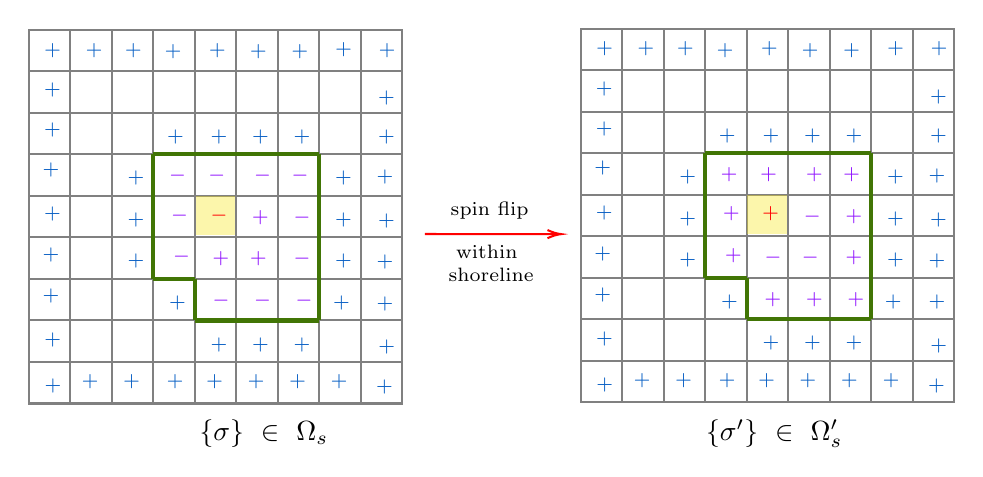
\begin{tikzpicture}[x=0.75pt,y=0.75pt,yscale=-1,xscale=1]
%uncomment if require: \path (0,239); %set diagram left start at 0, and has height of 239

%Shape: Grid [id:dp8379076404209189] 
\draw  [draw opacity=0] (15.17,18.64) -- (195.17,18.64) -- (195.17,198.64) -- (15.17,198.64) -- cycle ; \draw  [color={rgb, 255:red, 128; green, 128; blue, 128 }  ,draw opacity=1 ] (35.17,18.64) -- (35.17,198.64)(55.17,18.64) -- (55.17,198.64)(75.17,18.64) -- (75.17,198.64)(95.17,18.64) -- (95.17,198.64)(115.17,18.64) -- (115.17,198.64)(135.17,18.64) -- (135.17,198.64)(155.17,18.64) -- (155.17,198.64)(175.17,18.64) -- (175.17,198.64) ; \draw  [color={rgb, 255:red, 128; green, 128; blue, 128 }  ,draw opacity=1 ] (15.17,38.64) -- (195.17,38.64)(15.17,58.64) -- (195.17,58.64)(15.17,78.64) -- (195.17,78.64)(15.17,98.64) -- (195.17,98.64)(15.17,118.64) -- (195.17,118.64)(15.17,138.64) -- (195.17,138.64)(15.17,158.64) -- (195.17,158.64)(15.17,178.64) -- (195.17,178.64) ; \draw  [color={rgb, 255:red, 128; green, 128; blue, 128 }  ,draw opacity=1 ] (15.17,18.64) -- (195.17,18.64) -- (195.17,198.64) -- (15.17,198.64) -- cycle ;
%Straight Lines [id:da3742327723893828] 
\draw [color={rgb, 255:red, 65; green, 117; blue, 5 }  ,draw opacity=1 ][line width=1.5]    (75.17,78.64) -- (135.17,78.64) ;
%Straight Lines [id:da9396178230782906] 
\draw [color={rgb, 255:red, 65; green, 117; blue, 5 }  ,draw opacity=1 ][line width=1.5]    (155.17,78.64) -- (155.17,138.64) ;
%Straight Lines [id:da8719988645522738] 
\draw [color={rgb, 255:red, 65; green, 117; blue, 5 }  ,draw opacity=1 ][line width=1.5]    (155.17,78.64) -- (135.17,78.64) ;
%Straight Lines [id:da2329130725291969] 
\draw [color={rgb, 255:red, 65; green, 117; blue, 5 }  ,draw opacity=1 ][line width=1.5]    (155.17,158.64) -- (115.17,158.64) ;
%Straight Lines [id:da08515699568514723] 
\draw [color={rgb, 255:red, 65; green, 117; blue, 5 }  ,draw opacity=1 ][line width=1.5]    (155.17,138.64) -- (155.17,158.64) ;
%Straight Lines [id:da7105546115943345] 
\draw [color={rgb, 255:red, 65; green, 117; blue, 5 }  ,draw opacity=1 ][line width=1.5]    (95.17,158.64) -- (115.17,158.64) ;
%Straight Lines [id:da0002738983679971829] 
\draw [color={rgb, 255:red, 65; green, 117; blue, 5 }  ,draw opacity=1 ][line width=1.5]    (95.17,138.64) -- (95.17,158.64) ;
%Straight Lines [id:da6685411681475324] 
\draw [color={rgb, 255:red, 65; green, 117; blue, 5 }  ,draw opacity=1 ][line width=1.5]    (75.17,138.64) -- (75.17,78.64) ;
%Straight Lines [id:da07635822641625167] 
\draw [color={rgb, 255:red, 65; green, 117; blue, 5 }  ,draw opacity=1 ][line width=1.5]    (95.17,138.64) -- (75.17,138.64) ;
%Shape: Square [id:dp9422462087641228] 
\draw  [draw opacity=0][fill={rgb, 255:red, 248; green, 231; blue, 28 }  ,fill opacity=0.37 ] (95.55,98.55) -- (114.68,98.55) -- (114.68,117.68) -- (95.55,117.68) -- cycle ;
%Shape: Grid [id:dp5300081748363422] 
\draw  [draw opacity=0] (281.08,18.08) -- (461.08,18.08) -- (461.08,198.08) -- (281.08,198.08) -- cycle ; \draw  [color={rgb, 255:red, 128; green, 128; blue, 128 }  ,draw opacity=1 ] (301.08,18.08) -- (301.08,198.08)(321.08,18.08) -- (321.08,198.08)(341.08,18.08) -- (341.08,198.08)(361.08,18.08) -- (361.08,198.08)(381.08,18.08) -- (381.08,198.08)(401.08,18.08) -- (401.08,198.08)(421.08,18.08) -- (421.08,198.08)(441.08,18.08) -- (441.08,198.08) ; \draw  [color={rgb, 255:red, 128; green, 128; blue, 128 }  ,draw opacity=1 ] (281.08,38.08) -- (461.08,38.08)(281.08,58.08) -- (461.08,58.08)(281.08,78.08) -- (461.08,78.08)(281.08,98.08) -- (461.08,98.08)(281.08,118.08) -- (461.08,118.08)(281.08,138.08) -- (461.08,138.08)(281.08,158.08) -- (461.08,158.08)(281.08,178.08) -- (461.08,178.08) ; \draw  [color={rgb, 255:red, 128; green, 128; blue, 128 }  ,draw opacity=1 ] (281.08,18.08) -- (461.08,18.08) -- (461.08,198.08) -- (281.08,198.08) -- cycle ;
%Straight Lines [id:da5087420356242548] 
\draw [color={rgb, 255:red, 65; green, 117; blue, 5 }  ,draw opacity=1 ][line width=1.5]    (341.08,78.08) -- (401.08,78.08) ;
%Straight Lines [id:da48301607001523683] 
\draw [color={rgb, 255:red, 65; green, 117; blue, 5 }  ,draw opacity=1 ][line width=1.5]    (421.08,78.08) -- (421.08,138.08) ;
%Straight Lines [id:da47401257693283383] 
\draw [color={rgb, 255:red, 65; green, 117; blue, 5 }  ,draw opacity=1 ][line width=1.5]    (421.08,78.08) -- (401.08,78.08) ;
%Straight Lines [id:da5844334987470183] 
\draw [color={rgb, 255:red, 65; green, 117; blue, 5 }  ,draw opacity=1 ][line width=1.5]    (421.08,158.08) -- (381.08,158.08) ;
%Straight Lines [id:da7612907761119417] 
\draw [color={rgb, 255:red, 65; green, 117; blue, 5 }  ,draw opacity=1 ][line width=1.5]    (421.08,138.08) -- (421.08,158.08) ;
%Straight Lines [id:da6535580351469907] 
\draw [color={rgb, 255:red, 65; green, 117; blue, 5 }  ,draw opacity=1 ][line width=1.5]    (361.08,158.08) -- (381.08,158.08) ;
%Straight Lines [id:da7844570291759877] 
\draw [color={rgb, 255:red, 65; green, 117; blue, 5 }  ,draw opacity=1 ][line width=1.5]    (361.08,138.08) -- (361.08,158.08) ;
%Straight Lines [id:da5364070796173377] 
\draw [color={rgb, 255:red, 65; green, 117; blue, 5 }  ,draw opacity=1 ][line width=1.5]    (341.08,138.08) -- (341.08,78.08) ;
%Straight Lines [id:da273119584414117] 
\draw [color={rgb, 255:red, 65; green, 117; blue, 5 }  ,draw opacity=1 ][line width=1.5]    (361.08,138.08) -- (341.08,138.08) ;
%Shape: Square [id:dp445326990796883] 
\draw  [draw opacity=0][fill={rgb, 255:red, 248; green, 231; blue, 28 }  ,fill opacity=0.37 ] (361.47,97.99) -- (380.6,97.99) -- (380.6,117.13) -- (361.47,117.13) -- cycle ;
%Straight Lines [id:da7641152187991687] 
\draw [color={rgb, 255:red, 255; green, 0; blue, 0 }  ,draw opacity=1 ]   (206,117) -- (269.68,117.05) ;
\draw [shift={(271.68,117.05)}, rotate = 180.04] [color={rgb, 255:red, 255; green, 0; blue, 0 }  ,draw opacity=1 ][line width=0.75]    (6.56,-1.97) .. controls (4.17,-0.84) and (1.99,-0.18) .. (0,0) .. controls (1.99,0.18) and (4.17,0.84) .. (6.56,1.97)   ;

% Text Node
\draw (182.31,23.5) node [anchor=north west][inner sep=0.75pt]  [font=\scriptsize,color={rgb, 255:red, 9; green, 96; blue, 196 }  ,opacity=1 ]  {$+$};
% Text Node
\draw (101.17,103.04) node [anchor=north west][inner sep=0.75pt]  [font=\scriptsize,color={rgb, 255:red, 255; green, 0; blue, 0 }  ,opacity=1 ]  {$-$};
% Text Node
\draw (140.19,24.22) node [anchor=north west][inner sep=0.75pt]  [font=\scriptsize,color={rgb, 255:red, 9; green, 96; blue, 196 }  ,opacity=1 ]  {$+$};
% Text Node
\draw (100.53,23.5) node [anchor=north west][inner sep=0.75pt]  [font=\scriptsize,color={rgb, 255:red, 9; green, 96; blue, 196 }  ,opacity=1 ]  {$+$};
% Text Node
\draw (60.06,23.5) node [anchor=north west][inner sep=0.75pt]  [font=\scriptsize,color={rgb, 255:red, 9; green, 96; blue, 196 }  ,opacity=1 ]  {$+$};
% Text Node
\draw (21.08,23.5) node [anchor=north west][inner sep=0.75pt]  [font=\scriptsize,color={rgb, 255:red, 9; green, 96; blue, 196 }  ,opacity=1 ]  {$+$};
% Text Node
\draw (161.31,23.4) node [anchor=north west][inner sep=0.75pt]  [font=\scriptsize,color={rgb, 255:red, 9; green, 96; blue, 196 }  ,opacity=1 ]  {$+$};
% Text Node
\draw (120.19,24.22) node [anchor=north west][inner sep=0.75pt]  [font=\scriptsize,color={rgb, 255:red, 9; green, 96; blue, 196 }  ,opacity=1 ]  {$+$};
% Text Node
\draw (79.19,24.22) node [anchor=north west][inner sep=0.75pt]  [font=\scriptsize,color={rgb, 255:red, 9; green, 96; blue, 196 }  ,opacity=1 ]  {$+$};
% Text Node
\draw (41.06,23.5) node [anchor=north west][inner sep=0.75pt]  [font=\scriptsize,color={rgb, 255:red, 9; green, 96; blue, 196 }  ,opacity=1 ]  {$+$};
% Text Node
\draw (191.52,185.02) node [anchor=north west][inner sep=0.75pt]  [font=\scriptsize,color={rgb, 255:red, 9; green, 96; blue, 196 }  ,opacity=1 ,rotate=-90]  {$+$};
% Text Node
\draw (191.8,144.9) node [anchor=north west][inner sep=0.75pt]  [font=\scriptsize,color={rgb, 255:red, 9; green, 96; blue, 196 }  ,opacity=1 ,rotate=-90]  {$+$};
% Text Node
\draw (192.52,105.24) node [anchor=north west][inner sep=0.75pt]  [font=\scriptsize,color={rgb, 255:red, 9; green, 96; blue, 196 }  ,opacity=1 ,rotate=-90]  {$+$};
% Text Node
\draw (192.52,64.77) node [anchor=north west][inner sep=0.75pt]  [font=\scriptsize,color={rgb, 255:red, 9; green, 96; blue, 196 }  ,opacity=1 ,rotate=-90]  {$+$};
% Text Node
\draw (192.62,166.02) node [anchor=north west][inner sep=0.75pt]  [font=\scriptsize,color={rgb, 255:red, 9; green, 96; blue, 196 }  ,opacity=1 ,rotate=-90]  {$+$};
% Text Node
\draw (191.8,124.9) node [anchor=north west][inner sep=0.75pt]  [font=\scriptsize,color={rgb, 255:red, 9; green, 96; blue, 196 }  ,opacity=1 ,rotate=-90]  {$+$};
% Text Node
\draw (191.8,83.9) node [anchor=north west][inner sep=0.75pt]  [font=\scriptsize,color={rgb, 255:red, 9; green, 96; blue, 196 }  ,opacity=1 ,rotate=-90]  {$+$};
% Text Node
\draw (192.52,45.77) node [anchor=north west][inner sep=0.75pt]  [font=\scriptsize,color={rgb, 255:red, 9; green, 96; blue, 196 }  ,opacity=1 ,rotate=-90]  {$+$};
% Text Node
\draw (31.77,184.64) node [anchor=north west][inner sep=0.75pt]  [font=\scriptsize,color={rgb, 255:red, 9; green, 96; blue, 196 }  ,opacity=1 ,rotate=-90]  {$+$};
% Text Node
\draw (30.8,141.35) node [anchor=north west][inner sep=0.75pt]  [font=\scriptsize,color={rgb, 255:red, 9; green, 96; blue, 196 }  ,opacity=1 ,rotate=-90]  {$+$};
% Text Node
\draw (31.52,101.69) node [anchor=north west][inner sep=0.75pt]  [font=\scriptsize,color={rgb, 255:red, 9; green, 96; blue, 196 }  ,opacity=1 ,rotate=-90]  {$+$};
% Text Node
\draw (31.52,61.22) node [anchor=north west][inner sep=0.75pt]  [font=\scriptsize,color={rgb, 255:red, 9; green, 96; blue, 196 }  ,opacity=1 ,rotate=-90]  {$+$};
% Text Node
\draw (31.62,162.47) node [anchor=north west][inner sep=0.75pt]  [font=\scriptsize,color={rgb, 255:red, 9; green, 96; blue, 196 }  ,opacity=1 ,rotate=-90]  {$+$};
% Text Node
\draw (30.8,121.35) node [anchor=north west][inner sep=0.75pt]  [font=\scriptsize,color={rgb, 255:red, 9; green, 96; blue, 196 }  ,opacity=1 ,rotate=-90]  {$+$};
% Text Node
\draw (30.8,80.35) node [anchor=north west][inner sep=0.75pt]  [font=\scriptsize,color={rgb, 255:red, 9; green, 96; blue, 196 }  ,opacity=1 ,rotate=-90]  {$+$};
% Text Node
\draw (31.52,42.22) node [anchor=north west][inner sep=0.75pt]  [font=\scriptsize,color={rgb, 255:red, 9; green, 96; blue, 196 }  ,opacity=1 ,rotate=-90]  {$+$};
% Text Node
\draw (139.1,183.22) node [anchor=north west][inner sep=0.75pt]  [font=\scriptsize,color={rgb, 255:red, 9; green, 96; blue, 196 }  ,opacity=1 ]  {$+$};
% Text Node
\draw (99.17,183.04) node [anchor=north west][inner sep=0.75pt]  [font=\scriptsize,color={rgb, 255:red, 9; green, 96; blue, 196 }  ,opacity=1 ]  {$+$};
% Text Node
\draw (59.17,183.04) node [anchor=north west][inner sep=0.75pt]  [font=\scriptsize,color={rgb, 255:red, 9; green, 96; blue, 196 }  ,opacity=1 ]  {$+$};
% Text Node
\draw (159.17,183.04) node [anchor=north west][inner sep=0.75pt]  [font=\scriptsize,color={rgb, 255:red, 9; green, 96; blue, 196 }  ,opacity=1 ]  {$+$};
% Text Node
\draw (119.1,183.22) node [anchor=north west][inner sep=0.75pt]  [font=\scriptsize,color={rgb, 255:red, 9; green, 96; blue, 196 }  ,opacity=1 ]  {$+$};
% Text Node
\draw (80.1,183.22) node [anchor=north west][inner sep=0.75pt]  [font=\scriptsize,color={rgb, 255:red, 9; green, 96; blue, 196 }  ,opacity=1 ]  {$+$};
% Text Node
\draw (39.17,183.04) node [anchor=north west][inner sep=0.75pt]  [font=\scriptsize,color={rgb, 255:red, 9; green, 96; blue, 196 }  ,opacity=1 ]  {$+$};
% Text Node
\draw (171.77,124.64) node [anchor=north west][inner sep=0.75pt]  [font=\scriptsize,color={rgb, 255:red, 9; green, 96; blue, 196 }  ,opacity=1 ,rotate=-90]  {$+$};
% Text Node
\draw (170.77,144.64) node [anchor=north west][inner sep=0.75pt]  [font=\scriptsize,color={rgb, 255:red, 9; green, 96; blue, 196 }  ,opacity=1 ,rotate=-90]  {$+$};
% Text Node
\draw (171.77,104.64) node [anchor=north west][inner sep=0.75pt]  [font=\scriptsize,color={rgb, 255:red, 9; green, 96; blue, 196 }  ,opacity=1 ,rotate=-90]  {$+$};
% Text Node
\draw (171.77,84.64) node [anchor=north west][inner sep=0.75pt]  [font=\scriptsize,color={rgb, 255:red, 9; green, 96; blue, 196 }  ,opacity=1 ,rotate=-90]  {$+$};
% Text Node
\draw (151.77,64.64) node [anchor=north west][inner sep=0.75pt]  [font=\scriptsize,color={rgb, 255:red, 9; green, 96; blue, 196 }  ,opacity=1 ,rotate=-90]  {$+$};
% Text Node
\draw (131.77,64.64) node [anchor=north west][inner sep=0.75pt]  [font=\scriptsize,color={rgb, 255:red, 9; green, 96; blue, 196 }  ,opacity=1 ,rotate=-90]  {$+$};
% Text Node
\draw (111.77,64.64) node [anchor=north west][inner sep=0.75pt]  [font=\scriptsize,color={rgb, 255:red, 9; green, 96; blue, 196 }  ,opacity=1 ,rotate=-90]  {$+$};
% Text Node
\draw (90.77,64.64) node [anchor=north west][inner sep=0.75pt]  [font=\scriptsize,color={rgb, 255:red, 9; green, 96; blue, 196 }  ,opacity=1 ,rotate=-90]  {$+$};
% Text Node
\draw (71.77,84.64) node [anchor=north west][inner sep=0.75pt]  [font=\scriptsize,color={rgb, 255:red, 9; green, 96; blue, 196 }  ,opacity=1 ,rotate=-90]  {$+$};
% Text Node
\draw (71.77,104.64) node [anchor=north west][inner sep=0.75pt]  [font=\scriptsize,color={rgb, 255:red, 9; green, 96; blue, 196 }  ,opacity=1 ,rotate=-90]  {$+$};
% Text Node
\draw (91.77,144.64) node [anchor=north west][inner sep=0.75pt]  [font=\scriptsize,color={rgb, 255:red, 9; green, 96; blue, 196 }  ,opacity=1 ,rotate=-90]  {$+$};
% Text Node
\draw (71.77,124.64) node [anchor=north west][inner sep=0.75pt]  [font=\scriptsize,color={rgb, 255:red, 9; green, 96; blue, 196 }  ,opacity=1 ,rotate=-90]  {$+$};
% Text Node
\draw (111.77,164.64) node [anchor=north west][inner sep=0.75pt]  [font=\scriptsize,color={rgb, 255:red, 9; green, 96; blue, 196 }  ,opacity=1 ,rotate=-90]  {$+$};
% Text Node
\draw (131.77,164.64) node [anchor=north west][inner sep=0.75pt]  [font=\scriptsize,color={rgb, 255:red, 9; green, 96; blue, 196 }  ,opacity=1 ,rotate=-90]  {$+$};
% Text Node
\draw (151.77,164.64) node [anchor=north west][inner sep=0.75pt]  [font=\scriptsize,color={rgb, 255:red, 9; green, 96; blue, 196 }  ,opacity=1 ,rotate=-90]  {$+$};
% Text Node
\draw (82.17,103.04) node [anchor=north west][inner sep=0.75pt]  [font=\scriptsize,color={rgb, 255:red, 144; green, 19; blue, 254 }  ,opacity=1 ]  {$-$};
% Text Node
\draw (83.17,123.04) node [anchor=north west][inner sep=0.75pt]  [font=\scriptsize,color={rgb, 255:red, 144; green, 19; blue, 254 }  ,opacity=1 ]  {$-$};
% Text Node
\draw (102.17,144.04) node [anchor=north west][inner sep=0.75pt]  [font=\scriptsize,color={rgb, 255:red, 144; green, 19; blue, 254 }  ,opacity=1 ]  {$-$};
% Text Node
\draw (122.17,144.04) node [anchor=north west][inner sep=0.75pt]  [font=\scriptsize,color={rgb, 255:red, 144; green, 19; blue, 254 }  ,opacity=1 ]  {$-$};
% Text Node
\draw (142.17,144.04) node [anchor=north west][inner sep=0.75pt]  [font=\scriptsize,color={rgb, 255:red, 144; green, 19; blue, 254 }  ,opacity=1 ]  {$-$};
% Text Node
\draw (141.17,124.04) node [anchor=north west][inner sep=0.75pt]  [font=\scriptsize,color={rgb, 255:red, 144; green, 19; blue, 254 }  ,opacity=1 ]  {$-$};
% Text Node
\draw (141.17,104.04) node [anchor=north west][inner sep=0.75pt]  [font=\scriptsize,color={rgb, 255:red, 144; green, 19; blue, 254 }  ,opacity=1 ]  {$-$};
% Text Node
\draw (140.17,84.04) node [anchor=north west][inner sep=0.75pt]  [font=\scriptsize,color={rgb, 255:red, 144; green, 19; blue, 254 }  ,opacity=1 ]  {$-$};
% Text Node
\draw (122.17,84.04) node [anchor=north west][inner sep=0.75pt]  [font=\scriptsize,color={rgb, 255:red, 144; green, 19; blue, 254 }  ,opacity=1 ]  {$-$};
% Text Node
\draw (100.17,84.04) node [anchor=north west][inner sep=0.75pt]  [font=\scriptsize,color={rgb, 255:red, 144; green, 19; blue, 254 }  ,opacity=1 ]  {$-$};
% Text Node
\draw (81.17,84.04) node [anchor=north west][inner sep=0.75pt]  [font=\scriptsize,color={rgb, 255:red, 144; green, 19; blue, 254 }  ,opacity=1 ]  {$-$};
% Text Node
\draw (121.17,104.04) node [anchor=north west][inner sep=0.75pt]  [font=\scriptsize,color={rgb, 255:red, 144; green, 19; blue, 254 }  ,opacity=1 ]  {$+$};
% Text Node
\draw (120.17,124.04) node [anchor=north west][inner sep=0.75pt]  [font=\scriptsize,color={rgb, 255:red, 144; green, 19; blue, 254 }  ,opacity=1 ]  {$+$};
% Text Node
\draw (102.17,124.04) node [anchor=north west][inner sep=0.75pt]  [font=\scriptsize,color={rgb, 255:red, 144; green, 19; blue, 254 }  ,opacity=1 ]  {$+$};
% Text Node
\draw (448.22,22.95) node [anchor=north west][inner sep=0.75pt]  [font=\scriptsize,color={rgb, 255:red, 9; green, 96; blue, 196 }  ,opacity=1 ]  {$+$};
% Text Node
\draw (367.08,102.48) node [anchor=north west][inner sep=0.75pt]  [font=\scriptsize,color={rgb, 255:red, 255; green, 0; blue, 0 }  ,opacity=1 ]  {$+$};
% Text Node
\draw (406.1,23.67) node [anchor=north west][inner sep=0.75pt]  [font=\scriptsize,color={rgb, 255:red, 9; green, 96; blue, 196 }  ,opacity=1 ]  {$+$};
% Text Node
\draw (366.44,22.95) node [anchor=north west][inner sep=0.75pt]  [font=\scriptsize,color={rgb, 255:red, 9; green, 96; blue, 196 }  ,opacity=1 ]  {$+$};
% Text Node
\draw (325.97,22.95) node [anchor=north west][inner sep=0.75pt]  [font=\scriptsize,color={rgb, 255:red, 9; green, 96; blue, 196 }  ,opacity=1 ]  {$+$};
% Text Node
\draw (287,22.95) node [anchor=north west][inner sep=0.75pt]  [font=\scriptsize,color={rgb, 255:red, 9; green, 96; blue, 196 }  ,opacity=1 ]  {$+$};
% Text Node
\draw (427.22,22.84) node [anchor=north west][inner sep=0.75pt]  [font=\scriptsize,color={rgb, 255:red, 9; green, 96; blue, 196 }  ,opacity=1 ]  {$+$};
% Text Node
\draw (386.1,23.67) node [anchor=north west][inner sep=0.75pt]  [font=\scriptsize,color={rgb, 255:red, 9; green, 96; blue, 196 }  ,opacity=1 ]  {$+$};
% Text Node
\draw (345.1,23.67) node [anchor=north west][inner sep=0.75pt]  [font=\scriptsize,color={rgb, 255:red, 9; green, 96; blue, 196 }  ,opacity=1 ]  {$+$};
% Text Node
\draw (306.97,22.95) node [anchor=north west][inner sep=0.75pt]  [font=\scriptsize,color={rgb, 255:red, 9; green, 96; blue, 196 }  ,opacity=1 ]  {$+$};
% Text Node
\draw (457.43,184.47) node [anchor=north west][inner sep=0.75pt]  [font=\scriptsize,color={rgb, 255:red, 9; green, 96; blue, 196 }  ,opacity=1 ,rotate=-90]  {$+$};
% Text Node
\draw (457.71,144.35) node [anchor=north west][inner sep=0.75pt]  [font=\scriptsize,color={rgb, 255:red, 9; green, 96; blue, 196 }  ,opacity=1 ,rotate=-90]  {$+$};
% Text Node
\draw (458.43,104.69) node [anchor=north west][inner sep=0.75pt]  [font=\scriptsize,color={rgb, 255:red, 9; green, 96; blue, 196 }  ,opacity=1 ,rotate=-90]  {$+$};
% Text Node
\draw (458.43,64.22) node [anchor=north west][inner sep=0.75pt]  [font=\scriptsize,color={rgb, 255:red, 9; green, 96; blue, 196 }  ,opacity=1 ,rotate=-90]  {$+$};
% Text Node
\draw (458.54,165.47) node [anchor=north west][inner sep=0.75pt]  [font=\scriptsize,color={rgb, 255:red, 9; green, 96; blue, 196 }  ,opacity=1 ,rotate=-90]  {$+$};
% Text Node
\draw (457.71,124.35) node [anchor=north west][inner sep=0.75pt]  [font=\scriptsize,color={rgb, 255:red, 9; green, 96; blue, 196 }  ,opacity=1 ,rotate=-90]  {$+$};
% Text Node
\draw (457.71,83.35) node [anchor=north west][inner sep=0.75pt]  [font=\scriptsize,color={rgb, 255:red, 9; green, 96; blue, 196 }  ,opacity=1 ,rotate=-90]  {$+$};
% Text Node
\draw (458.43,45.22) node [anchor=north west][inner sep=0.75pt]  [font=\scriptsize,color={rgb, 255:red, 9; green, 96; blue, 196 }  ,opacity=1 ,rotate=-90]  {$+$};
% Text Node
\draw (297.68,184.08) node [anchor=north west][inner sep=0.75pt]  [font=\scriptsize,color={rgb, 255:red, 9; green, 96; blue, 196 }  ,opacity=1 ,rotate=-90]  {$+$};
% Text Node
\draw (296.71,140.79) node [anchor=north west][inner sep=0.75pt]  [font=\scriptsize,color={rgb, 255:red, 9; green, 96; blue, 196 }  ,opacity=1 ,rotate=-90]  {$+$};
% Text Node
\draw (297.43,101.13) node [anchor=north west][inner sep=0.75pt]  [font=\scriptsize,color={rgb, 255:red, 9; green, 96; blue, 196 }  ,opacity=1 ,rotate=-90]  {$+$};
% Text Node
\draw (297.43,60.66) node [anchor=north west][inner sep=0.75pt]  [font=\scriptsize,color={rgb, 255:red, 9; green, 96; blue, 196 }  ,opacity=1 ,rotate=-90]  {$+$};
% Text Node
\draw (297.54,161.91) node [anchor=north west][inner sep=0.75pt]  [font=\scriptsize,color={rgb, 255:red, 9; green, 96; blue, 196 }  ,opacity=1 ,rotate=-90]  {$+$};
% Text Node
\draw (296.71,120.79) node [anchor=north west][inner sep=0.75pt]  [font=\scriptsize,color={rgb, 255:red, 9; green, 96; blue, 196 }  ,opacity=1 ,rotate=-90]  {$+$};
% Text Node
\draw (296.71,79.79) node [anchor=north west][inner sep=0.75pt]  [font=\scriptsize,color={rgb, 255:red, 9; green, 96; blue, 196 }  ,opacity=1 ,rotate=-90]  {$+$};
% Text Node
\draw (297.43,41.66) node [anchor=north west][inner sep=0.75pt]  [font=\scriptsize,color={rgb, 255:red, 9; green, 96; blue, 196 }  ,opacity=1 ,rotate=-90]  {$+$};
% Text Node
\draw (405.02,182.67) node [anchor=north west][inner sep=0.75pt]  [font=\scriptsize,color={rgb, 255:red, 9; green, 96; blue, 196 }  ,opacity=1 ]  {$+$};
% Text Node
\draw (365.08,182.48) node [anchor=north west][inner sep=0.75pt]  [font=\scriptsize,color={rgb, 255:red, 9; green, 96; blue, 196 }  ,opacity=1 ]  {$+$};
% Text Node
\draw (325.08,182.48) node [anchor=north west][inner sep=0.75pt]  [font=\scriptsize,color={rgb, 255:red, 9; green, 96; blue, 196 }  ,opacity=1 ]  {$+$};
% Text Node
\draw (425.08,182.48) node [anchor=north west][inner sep=0.75pt]  [font=\scriptsize,color={rgb, 255:red, 9; green, 96; blue, 196 }  ,opacity=1 ]  {$+$};
% Text Node
\draw (385.02,182.67) node [anchor=north west][inner sep=0.75pt]  [font=\scriptsize,color={rgb, 255:red, 9; green, 96; blue, 196 }  ,opacity=1 ]  {$+$};
% Text Node
\draw (346.02,182.67) node [anchor=north west][inner sep=0.75pt]  [font=\scriptsize,color={rgb, 255:red, 9; green, 96; blue, 196 }  ,opacity=1 ]  {$+$};
% Text Node
\draw (305.08,182.48) node [anchor=north west][inner sep=0.75pt]  [font=\scriptsize,color={rgb, 255:red, 9; green, 96; blue, 196 }  ,opacity=1 ]  {$+$};
% Text Node
\draw (437.68,124.08) node [anchor=north west][inner sep=0.75pt]  [font=\scriptsize,color={rgb, 255:red, 9; green, 96; blue, 196 }  ,opacity=1 ,rotate=-90]  {$+$};
% Text Node
\draw (436.68,144.08) node [anchor=north west][inner sep=0.75pt]  [font=\scriptsize,color={rgb, 255:red, 9; green, 96; blue, 196 }  ,opacity=1 ,rotate=-90]  {$+$};
% Text Node
\draw (437.68,104.08) node [anchor=north west][inner sep=0.75pt]  [font=\scriptsize,color={rgb, 255:red, 9; green, 96; blue, 196 }  ,opacity=1 ,rotate=-90]  {$+$};
% Text Node
\draw (437.68,84.08) node [anchor=north west][inner sep=0.75pt]  [font=\scriptsize,color={rgb, 255:red, 9; green, 96; blue, 196 }  ,opacity=1 ,rotate=-90]  {$+$};
% Text Node
\draw (417.68,64.08) node [anchor=north west][inner sep=0.75pt]  [font=\scriptsize,color={rgb, 255:red, 9; green, 96; blue, 196 }  ,opacity=1 ,rotate=-90]  {$+$};
% Text Node
\draw (397.68,64.08) node [anchor=north west][inner sep=0.75pt]  [font=\scriptsize,color={rgb, 255:red, 9; green, 96; blue, 196 }  ,opacity=1 ,rotate=-90]  {$+$};
% Text Node
\draw (377.68,64.08) node [anchor=north west][inner sep=0.75pt]  [font=\scriptsize,color={rgb, 255:red, 9; green, 96; blue, 196 }  ,opacity=1 ,rotate=-90]  {$+$};
% Text Node
\draw (356.68,64.08) node [anchor=north west][inner sep=0.75pt]  [font=\scriptsize,color={rgb, 255:red, 9; green, 96; blue, 196 }  ,opacity=1 ,rotate=-90]  {$+$};
% Text Node
\draw (337.68,84.08) node [anchor=north west][inner sep=0.75pt]  [font=\scriptsize,color={rgb, 255:red, 9; green, 96; blue, 196 }  ,opacity=1 ,rotate=-90]  {$+$};
% Text Node
\draw (337.68,104.08) node [anchor=north west][inner sep=0.75pt]  [font=\scriptsize,color={rgb, 255:red, 9; green, 96; blue, 196 }  ,opacity=1 ,rotate=-90]  {$+$};
% Text Node
\draw (357.68,144.08) node [anchor=north west][inner sep=0.75pt]  [font=\scriptsize,color={rgb, 255:red, 9; green, 96; blue, 196 }  ,opacity=1 ,rotate=-90]  {$+$};
% Text Node
\draw (337.68,124.08) node [anchor=north west][inner sep=0.75pt]  [font=\scriptsize,color={rgb, 255:red, 9; green, 96; blue, 196 }  ,opacity=1 ,rotate=-90]  {$+$};
% Text Node
\draw (377.68,164.08) node [anchor=north west][inner sep=0.75pt]  [font=\scriptsize,color={rgb, 255:red, 9; green, 96; blue, 196 }  ,opacity=1 ,rotate=-90]  {$+$};
% Text Node
\draw (397.68,164.08) node [anchor=north west][inner sep=0.75pt]  [font=\scriptsize,color={rgb, 255:red, 9; green, 96; blue, 196 }  ,opacity=1 ,rotate=-90]  {$+$};
% Text Node
\draw (417.68,164.08) node [anchor=north west][inner sep=0.75pt]  [font=\scriptsize,color={rgb, 255:red, 9; green, 96; blue, 196 }  ,opacity=1 ,rotate=-90]  {$+$};
% Text Node
\draw (348.08,102.48) node [anchor=north west][inner sep=0.75pt]  [font=\scriptsize,color={rgb, 255:red, 144; green, 19; blue, 254 }  ,opacity=1 ]  {$+$};
% Text Node
\draw (349.08,122.48) node [anchor=north west][inner sep=0.75pt]  [font=\scriptsize,color={rgb, 255:red, 144; green, 19; blue, 254 }  ,opacity=1 ]  {$+$};
% Text Node
\draw (368.08,143.48) node [anchor=north west][inner sep=0.75pt]  [font=\scriptsize,color={rgb, 255:red, 144; green, 19; blue, 254 }  ,opacity=1 ]  {$+$};
% Text Node
\draw (388.08,143.48) node [anchor=north west][inner sep=0.75pt]  [font=\scriptsize,color={rgb, 255:red, 144; green, 19; blue, 254 }  ,opacity=1 ]  {$+$};
% Text Node
\draw (408.08,143.48) node [anchor=north west][inner sep=0.75pt]  [font=\scriptsize,color={rgb, 255:red, 144; green, 19; blue, 254 }  ,opacity=1 ]  {$+$};
% Text Node
\draw (407.08,123.48) node [anchor=north west][inner sep=0.75pt]  [font=\scriptsize,color={rgb, 255:red, 144; green, 19; blue, 254 }  ,opacity=1 ]  {$+$};
% Text Node
\draw (407.08,103.48) node [anchor=north west][inner sep=0.75pt]  [font=\scriptsize,color={rgb, 255:red, 144; green, 19; blue, 254 }  ,opacity=1 ]  {$+$};
% Text Node
\draw (406.08,83.48) node [anchor=north west][inner sep=0.75pt]  [font=\scriptsize,color={rgb, 255:red, 144; green, 19; blue, 254 }  ,opacity=1 ]  {$+$};
% Text Node
\draw (388.08,83.48) node [anchor=north west][inner sep=0.75pt]  [font=\scriptsize,color={rgb, 255:red, 144; green, 19; blue, 254 }  ,opacity=1 ]  {$+$};
% Text Node
\draw (366.08,83.48) node [anchor=north west][inner sep=0.75pt]  [font=\scriptsize,color={rgb, 255:red, 144; green, 19; blue, 254 }  ,opacity=1 ]  {$+$};
% Text Node
\draw (347.08,83.48) node [anchor=north west][inner sep=0.75pt]  [font=\scriptsize,color={rgb, 255:red, 144; green, 19; blue, 254 }  ,opacity=1 ]  {$+$};
% Text Node
\draw (387.08,103.48) node [anchor=north west][inner sep=0.75pt]  [font=\scriptsize,color={rgb, 255:red, 144; green, 19; blue, 254 }  ,opacity=1 ]  {$-$};
% Text Node
\draw (386.08,123.48) node [anchor=north west][inner sep=0.75pt]  [font=\scriptsize,color={rgb, 255:red, 144; green, 19; blue, 254 }  ,opacity=1 ]  {$-$};
% Text Node
\draw (368.08,123.48) node [anchor=north west][inner sep=0.75pt]  [font=\scriptsize,color={rgb, 255:red, 144; green, 19; blue, 254 }  ,opacity=1 ]  {$-$};
% Text Node
\draw (217,100) node [anchor=north west][inner sep=0.75pt]  [font=\scriptsize] [align=left] {spin flip};
% Text Node
\draw (216,121) node [anchor=north west][inner sep=0.75pt]  [font=\scriptsize] [align=left] { \ within \\shoreline};
% Text Node
\draw (96,204.77) node [anchor=north west][inner sep=0.75pt]    {$\{\sigma \} \ \in \ \Omega _{s}$};
% Text Node
\draw (340,204.87) node [anchor=north west][inner sep=0.75pt]    {$\{\sigma '\} \ \in \ \Omega '_{s}$};


\end{tikzpicture}

    \caption{Flipping of all the spins inside the shoreline, taking $\sigma\to \sigma'$}
    \label{peirl4}
\end{figure}
\noindent
We consider a specific configuration $\{\sigma\}\in \Omega\tund{s}$ and then flip all the spins in the inner side of the shoreline as shown in Fig. \ref{peirl4}. We call this configuration $\{\sigma'\}$. If a spin in this configuration is outside the shoreline, then $\sigma_i = \sigma'_i$ since the spins outside the shoreline remains unchanged. If the spins belong inside the shoreline, then both spins have flipped and we have $\sigma_i'\sigma_j' = (-\sigma_i) (-\sigma_j) = \sigma_i\sigma_j$. If the spins are separated by shoreline, only one of the spins (which is in the inner side of the shoreline ) changes and $\sigma_i'\sigma_j' = -\sigma_i \sigma_j = -(-1)=+1$. Thus we have,
$$\sum\limits_{\avg{ij}}\sigma_i' \sigma_j ' = \sum\limits_{\avg{ij}\in S}\sigma_i' \sigma_j '+\sum\limits_{\avg{ij}\notin S}\sigma_i' \sigma_j ' = n(S)+\sum\limits_{\avg{ij}\notin S}\sigma_i \sigma_j$$
Note that $n(S)>0$ always which give us the inequality,
$$\sum\limits_{\avg{ij}\notin S} \sigma_i \sigma_j =\sum\limits_{\avg{ij}}\sigma_i' \sigma_j ' - n(S) <\sum\limits_{\avg{ij}}\sigma_i' \sigma_j '$$ 
Also note that $\sigma_i\to \sigma'_i$ is a one-to-one map and hence the sum of spins over $\Omega\tund{s}$ is equal to the sum of spins over $\Omega'\tund{s}$. Using this and the estimate of the sum, Eq. \eqref{probdw} becomes, 
\begin{align}
    \begin{split}
        \mathrm{Prob}(\{\sigma\}\in \Omega\tund{s}) &< \frac{1}{\SZ}\sum\limits_{\{\sigma'\}\in\Omega'\tund{s}} e^{-\beta J n(S)} \exp\qty[\beta J \sum\limits_{\avg{ij}}\sigma_i'\sigma_j']\\
        &=\frac{e^{-\beta J n(S)}}{\SZ}\sum\limits_{\{\sigma'\}\in\Omega'\tund{s}}  \exp\qty[\beta J \sum\limits_{\avg{ij}}\sigma_i'\sigma_j']
    \end{split}
\end{align}
Now, the RHS is the sum over all configurations in $\Omega'\tund{s}$. Since $e^x>0$ for all $x$, this term is less than the sum over all the configurations $\{\sigma\}\in \Omega$. Thus,
$$ \mathrm{Prob}(\{\sigma\}\in \Omega\tund{s}) < e^{-\beta J n(S)}\frac{1}{\SZ} \mathcolor{red}{\sum\limits_{\{\sigma\}\in \Omega} \exp\qty[\beta J \sum\limits_{\avg{ij}}\sigma_i\sigma_j]} = e^{-\beta J n(S)}$$
since the red term is just the definition of the partition function. Thus the probability of any configuration in $\Omega\tund{s}$ is less than $e^{-\beta Jn(S)}$. However, we were interested in the situation where the configuration belonged to $\Omega\tund{0}$ which can be obtained by summing over all such possible shorelines $S$. 
\begin{align*}
    \mathrm{Prob}(\{\sigma\} \in \Omega\tund{0}) =\sum\limits_{\{S \}}\mathrm{Prob}(\Omega\tund{S})< \sum\limits_{\{S\}} e^{-\beta J n(S)}
\end{align*}
Note that the length $n$ of a shoreline can be $n=4,5,6\ldots$. The minimum value is $4$, for the shoreline which contains only the central spin and this length increases. Then the sum over shorelines can be written as, 
$$\mathrm{Prob}(\{\sigma\} \in \Omega\tund{0}) <\sum\limits_{n=4}^\infty s(n) e^{-\beta J n}$$
where $s(n)$ denote the number of shorelines with length $n$. The final thing to do is to have an estimate for $s(n)$. For this, note that shorelines are closed curves. To form a shoreline, start from any point $P$. We can move in only three directions (not in four) since shorelines are self-avoiding, so we cannot move in the direction in which we had already formed a line.\\[0.2cm] The number of ways to form a shoreline of length $n$ is thus $\sim 3^n$. Note that in this case, the choice of $P$ was arbitrary and we can essentially start from any of the $n$ points. Thus, the number of shorelines of length $n$ is $s(n)\sim 3^n n$. Substituting this in the above expression, 
$$\mathrm{Prob}(\{\sigma\} \in \Omega\tund{0}) <\sum\limits_{n=4}^\infty  3^n ne^{-\beta J n} \equiv\sum\limits_{n=4}^\infty  n r^n <\sum\limits_{n=1}^\infty  n r^n \qquad \text{where, }r =3e^{-\beta J }$$
From the ratio test, we have 
$$\lim\limits_{k\to \infty}\abs{\frac{a_{k+1}}{a_k}} = \lim\limits_{k\to \infty}\abs{\frac{(k+1)r^{k+1}}{kr^k}} =\lim\limits_{k\to \infty}\qty(1+\frac{1}{k})\abs{r} = \abs{r}$$
and hence the sum converges if $\abs{r}<1\implies e^{\beta J}>3$. The value of the sum in the RHS is $\frac{r}{(r-1)^2}$ and hence,
$$\mathrm{Prob}(\{\sigma\} \in \Omega\tund{0}) < \frac{r}{(r-1)^2} = \frac{3e^{-\beta J }}{(3e^{-\beta J }-1)^2}$$
As $\beta\to \infty$ (corresponding to $T\to 0$), $\mathrm{Prob}(\{\sigma\} \in \Omega\tund{0}) \to 0$ and hence for sufficiently low temperatures all spins in the systems tend to align even without an external magnetic field, proving the existence of a phase transition. 
\subsection{Symmetries of the Ising Model}
The zero-field Ising Hamiltonian has an obvious symmetry of $\sigma_i \mapsto -\sigma_i$, which is broken if $h\neq 0$. In non-zero field, from Eq. \eqref{isingham}, we can see that if $h\to -h$ and $\{\sigma\}\to \{-\sigma\}$, then the Ising Hamiltonian remains invariant. 
$$\SH(J, h, \{\sigma\}) = \SH(J,-h,\{-\sigma\})$$
This is called the \textit{time-reversal} symmetry or $\inte_2$ symmetry. Let us see what happens to the partition function under $h\to -h$. 
\begin{align*}
    \SZ(-h, J, T) &= \sum\limits_{\{\sigma\}} \exp\qty[-\beta \SH(-h, J,\{\sigma\})]\\
    &=\sum\limits_{\{\sigma\}} \exp\qty[-\beta\SH(-h, J,\{-\sigma\})]\\
    &=\sum\limits_{\{\sigma\}} \exp\qty[-\beta\SH(h, J,\{\sigma\})]=\SZ(h,J,T)
\end{align*}
where in the second sum we used the fact that changing $\sigma\to -\sigma$ will not matter since we are summing over both $-1$ and $+1$ spins. The free energy is just the logarithm of the partition function, hence it also enjoys the symmetry,
$$F(-h, J, T) = F(h, J,T)$$
From the free energy, we obtain the magnetisation  
\begin{align}
    \begin{split}
        \SM(h) = -\pdv{F(h,J,T)}{h} = -\pdv{F(-h,J,T)}{h} = \pdv{F(-h,J,T)}{(-h)} = -\SM(-h)
    \end{split}
\end{align} 
From the above expression, if $h=0$ then we have $\SM(0) = 0$ which apparently says that \textit{phase transition is impossible in zero-field!}\\[0.2cm]
This situation arises since we assumed the derivative of the free energy is well-behaved which is indeed true for finite systems, however, in the thermodynamic limit, $F$ develops a \text{kink} for $T<T_c$ and hence $\qty(\pdv{F}{h})$ develops a discontinuity as shown in Fig. \ref{kink} (a)
\begin{figure}[H]
    \centering 
    

\tikzset{every picture/.style={line width=0.75pt}} %set default line width to 0.75pt        

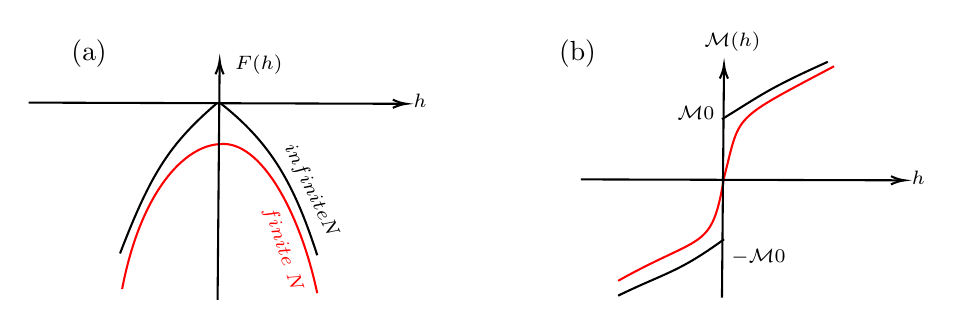
\begin{tikzpicture}[x=0.75pt,y=0.75pt,yscale=-1,xscale=1]
%uncomment if require: \path (0,170); %set diagram left start at 0, and has height of 170

%Straight Lines [id:da23635493997133195] 
\draw    (59,49) -- (239,49.58) ;
\draw [shift={(241,49.58)}, rotate = 180.18] [color={rgb, 255:red, 0; green, 0; blue, 0 }  ][line width=0.75]    (6.56,-1.97) .. controls (4.17,-0.84) and (1.99,-0.18) .. (0,0) .. controls (1.99,0.18) and (4.17,0.84) .. (6.56,1.97)   ;
%Curve Lines [id:da18235450228974837] 
\draw    (151,49) .. controls (176,68.52) and (187,88.52) .. (198,122.52) ;
%Curve Lines [id:da1225976391320428] 
\draw    (150,49) .. controls (127,68.8) and (118,82.67) .. (103,121.67) ;
%Curve Lines [id:da22793112325804687] 
\draw [color={rgb, 255:red, 255; green, 0; blue, 0 }  ,draw opacity=1 ]   (151,69) .. controls (171,66.8) and (190,102.8) .. (198,140.8) ;
%Curve Lines [id:da9488433252498562] 
\draw [color={rgb, 255:red, 255; green, 0; blue, 0 }  ,draw opacity=1 ]   (151,69) .. controls (134,69.8) and (113,91.8) .. (104,138.8) ;
%Straight Lines [id:da1517918266482663] 
\draw    (150,144) -- (150.98,30.8) ;
\draw [shift={(151,28.8)}, rotate = 90.5] [color={rgb, 255:red, 0; green, 0; blue, 0 }  ][line width=0.75]    (6.56,-1.97) .. controls (4.17,-0.84) and (1.99,-0.18) .. (0,0) .. controls (1.99,0.18) and (4.17,0.84) .. (6.56,1.97)   ;
%Curve Lines [id:da2541371388654118] 
\draw [color={rgb, 255:red, 255; green, 0; blue, 0 }  ,draw opacity=1 ]   (394,85.2) .. controls (402,54) and (397,58) .. (447,31.5) ;
%Curve Lines [id:da026300410741942226] 
\draw [color={rgb, 255:red, 255; green, 0; blue, 0 }  ,draw opacity=1 ]   (343,134.85) .. controls (384,111.85) and (388,120.85) .. (394,85.2) ;
%Curve Lines [id:da30742639571825414] 
\draw    (393,57) .. controls (412,45.35) and (415,42.35) .. (444,29.35) ;
%Curve Lines [id:da21107772902168997] 
\draw    (343,142) .. controls (366,130.85) and (372,130.85) .. (394,114.85) ;
%Straight Lines [id:da4537306814275738] 
\draw    (393,143) -- (393.98,32.85) ;
\draw [shift={(394,30.85)}, rotate = 90.51] [color={rgb, 255:red, 0; green, 0; blue, 0 }  ][line width=0.75]    (6.56,-1.97) .. controls (4.17,-0.84) and (1.99,-0.18) .. (0,0) .. controls (1.99,0.18) and (4.17,0.84) .. (6.56,1.97)   ;
%Straight Lines [id:da838604604323268] 
\draw    (325,86) -- (479,86.44) ;
\draw [shift={(481,86.45)}, rotate = 180.17] [color={rgb, 255:red, 0; green, 0; blue, 0 }  ][line width=0.75]    (6.56,-1.97) .. controls (4.17,-0.84) and (1.99,-0.18) .. (0,0) .. controls (1.99,0.18) and (4.17,0.84) .. (6.56,1.97)   ;

% Text Node
\draw (157,24.4) node [anchor=north west][inner sep=0.75pt]  [font=\scriptsize]  {$F( h)$};
% Text Node
\draw (243,43.4) node [anchor=north west][inner sep=0.75pt]  [font=\scriptsize]  {$h$};
% Text Node
\draw (179.57,96.47) node [anchor=north west][inner sep=0.75pt]  [font=\scriptsize,color={rgb, 255:red, 255; green, 0; blue, 0 }  ,opacity=1 ,rotate=-71.4]  {$\text{finite} \ N$};
% Text Node
\draw (188.7,65.63) node [anchor=north west][inner sep=0.75pt]  [font=\scriptsize,color={rgb, 255:red, 0; green, 0; blue, 0 }  ,opacity=1 ,rotate=-64.07]  {$\text{infinite } N$};
% Text Node
\draw (483,80.4) node [anchor=north west][inner sep=0.75pt]  [font=\scriptsize]  {$h$};
% Text Node
\draw (383,13.4) node [anchor=north west][inner sep=0.75pt]  [font=\scriptsize]  {$\mathcal{M}( h)$};
% Text Node
\draw (370,49.4) node [anchor=north west][inner sep=0.75pt]  [font=\scriptsize]  {$\mathcal{M}\tund{0}$};
% Text Node
\draw (396,118.25) node [anchor=north west][inner sep=0.75pt]  [font=\scriptsize]  {$-\mathcal{M}\tund{0}$};
% Text Node
\draw (78,17) node [anchor=north west][inner sep=0.75pt]   [align=left] {(a)};
% Text Node
\draw (313,17) node [anchor=north west][inner sep=0.75pt]   [align=left] {(b)};


\end{tikzpicture}

    \caption{(a) Free energy and (b) Magnetisation behaviour in finite $N$ and thermodynamic limit for $T<T_c$.}
    \label{kink}
\end{figure}
\noindent
In the thermodynamic limit, near $h=0$ the free energy behaves as,
$$F(h) = F(0) - \SM\tund{0} \abs{h} +\SO(h^{q>1})$$
From this, if $h<0$ then $\SM(0^-) = -\SM\tund{0}$ and if $h>0$ then $\SM(0^+) = +\SM\tund{0}$ which is clearly discontinuous as shown in Fig. \ref{kink} (b). It is clear that if we take the thermodynamic limit first and then take $h\to 0$ and if we first take $h\to 0$ for a finite $N$ and then take $N\to infty$, we get two different behaviours. Thus, the limits do not commute.  
$$\lim\limits_{N\to\infty}\lim\limits_{h\to 0} \qty( \frac{1}{N}\pdv{F(h)}{h})\neq \lim\limits_{h\to 0}\lim\limits_{N\to\infty} \qty( \frac{1}{N}\pdv{F(h)}{h})$$ 
\subsubsection{Spontaneous Symmetry Breaking}
When the Hamiltonian of the system has a particular symmetry but the statistical behavior of the system breaks that symmetry, we say that the symmetry is broken spontaneously. As seen before, the zero-field Ising Hamiltonian enjoys a $\inte_2$ symmetry, under the exchange $\{\sigma_i \}\to \{-\sigma_i\}$. For $T<T_c$ in the thermodynamic limit, we saw that 
$$m = \lim\limits_{N\to \infty} \frac{1}{N}\sum\limits_i \avg{\sigma_i} \neq 0$$
Hence, at all temperature $\SH$ has a symmetry under the exchange of spins but $\avg{\sigma_i}$ does not. Thus we say that the symmetry is spontaneously broken.\\[0.2cm]
This is different from the uninteresting explicit symmetry breaking in the $h\neq 0$ case, where the Hamiltonian itself does not have the $\inte_2$ symmetry from beginning.\\[0.2cm]
Spontaneous symmetry breaking seems a bit counterintuitive if we naively see a probabilistic viewpoint of the situation. Since the Hamiltonian has $\inte_2$ symmetry, the Boltzmann factor $P(\{\sigma\}) = \frac{1}{\SZ}\exp\qty(-\beta \SH(\{\sigma\}))$ is also invariant under this symmetry. Then the expectation, 
\begin{align*}
    \avg{\sigma_i} = \sum\limits_{\{\sigma\}}\sigma_i P(\{\sigma\}) = 0 
\end{align*}
The sum is zero because for a configuration $\{\sigma_i\}$, the opposite configuration $\{-\sigma_i\}$ will have the same Boltzmann factor, however, the $\sigma_i$ factor in the sum will become $-\sigma_i$, which will cancel with the configuration. Thus, in the thermodynamic limit, we have to be careful with the calculation!\\[0.2cm]
Consider the Ising model when $h\neq 0$. In this case, consider two configurations $A$ and $B$ which differ by the fact that all spins in configuration $B$ are the flipped spins of configuration $A$. Due to the field term $-h\sum \sigma_i = -hNm$, the probability of these two contributions will be
$$\frac{P\tund{A}}{P\tund{B}} = \frac{\exp[\beta h N m ]}{\exp[-\beta h N m ]} \implies \frac{P\tund{B}}{P\tund{A}} = \exp[-2\beta h N m ]$$
In the thermodynamic limit, for $h>0$, $\frac{P\tund{B}}{P\tund{A}} \to 0$ and hence the system must be in configuration $A$, with magnetisation $+m$ for any $h>0$ (in particular, true for $h\to 0^+$). For $h<0$, $\frac{P\tund{B}}{P\tund{A}}\to \infty $ and hence the system must be in configuration $B$, with magnetisation $-m$ for any $h<0$ (in particular, true for $h\to 0^-$).\\[0.2cm] Thus, in an infinitesimal field close to zero and in the thermodynamic limit, there is a large weight assigned to states with particular magnetisation $+m$ or $-m$, for $h>0$ and $h<0$ respectively. This is equivalent to setting $h=0$ but taking a \textit{restricted ensemble}, where we exclude the configurations with the `unpreferred' magnetisation and thus, their Boltzmann weight is identically zero. Two such probability distribution can be defined $P_+$ and $P_-$ based on the magnetisation values. I haven't gone through the rigorous mathematical arguments for this, however, Goldenfeld advised to refer to \cite{Glimm}, where this has been dealt with rigorously.